\documentclass[12pt, ngerman]{article}

\usepackage[a4paper, inner=2.5cm, outer=2.5cm, top=2.5cm, bottom=2cm, bindingoffset=0cm]{geometry}

\title{\Large{\textbf{3D-Tracking-System auf Basis herkömmlicher Kameras}}}
\author{Alexander Minor}

% text input
\usepackage[utf8]{inputenc}
\newcommand\Kurzfassung{Das Ziel unseres Projektes ist es, eine robuste, zuverlässige, modulare, 3D-gedruckte und einfach zu bedienende Unterwassersonde zu designen und mit einem elektrischen System auszustatten, welches mit diversen Sensoren Daten für die spätere graphische Visualisierung und Analyse sammelt. Wir erarbeiteten zunächst verschiedene Konzepte für das Hauptmodul, kombinierten ihre Vorteile und begannen mit dem Entwicklungsprozess der Sonde. Zuerst testeten wir kritische und komplexe Teile in kleinen Prototypen, wie Luke, Fenster und Wandstruktur. Diese und alle weiteren Modelle druckten wir in unserem durch Spenden finanzierten 3D-Drucker. Da diese von allein aufgrund der Struktur von 3D-gedrucktem Plastik nicht dicht sind, testeten wir im Laufe des Projektes verschiede chemische Überarbeitungstechniken mit Lack und Epoxidharz. Nachdem wir nun also alle wichtigen Teile der Sonde getestet haben, setzten wir uns an unseren ersten kompletten Prototypen, der sich in einem Schwimmbad Test ohne Elektronik als teilweise undicht erwiesen hat. Trotzdem zeigte uns dieser Tauchgang einige Aspekte auf, die noch überarbeitet werden müssten. Beim nächsten Prototyp veränderten wir die Position der druckaushaltenden Wandstruktur, die Luke und entwickelten ein neues modulares Verbindungssystem aus Gewindestangen. Dieser konnte sich in einem zweiten Schwimmbad Test beweisen, wie auch unsere Elektronikeinheit und unser Wasserprobenmodul.}
\newcommand\Einleitung{Bemannte Tauchgänge in die Tiefe von Gewässern sind meist umständlich, kompliziert, bergen ein hohes Risiko und sind vor allem teuer. Trotzdem ist es in vielen Situationen in Wirtschaft und Forschung notwendig, dass gewisse Aktionen und Datenmessungen tief unter dem Meeresspiegel stattfinden. Deshalb kommen immer mehr moderne Tauchsonden oder auch Tauchroboter zum Einsatz, welche je nach Notwendigkeit den Druck aushalten und somit auch wasserfest sein müssen, um Elektronik und Messgeräte in dieser Umgebung zu schützen. Diese Tauchsonden können meist autonom oder ferngesteuert die Aufgaben bewerkstelligen, sodass die Entwicklung dieser in den letzten Jahren und Jahrzehnten immer mehr an Relevanz gewonnen hat.}
\newcommand\StandEntwicklung{Unterwassersonden und Drohnen haben und werden auch in der Zukunft noch größeren Nutzen in Wirtschaft und Forschung haben. \par
Die Meeresböden der Ozeane in bestimmten Regionen bergen das Potenzial einer wichtigen Rohstoffquelle für wichtige Erze wie Kobalt, Kupfer und Nickel, welche hohe Nachfrage erfahren, da sie essenziell für moderne Technik sind und derzeitige Quellen aufgrund schlechter Arbeitsbedingungen und Ausbeutung an Attraktivität verlieren. In diesen Gebieten lassen sich tief unter der Wasseroberfläche ganze Felder an sogenannten Manganknollen finden, ballähnliche Metallklumpen, welche unter anderem die genannten Rohstoffe enthalten. Bisher war der „Abbau“ jedoch aus Umweltschutzgründen nicht möglich, da vorherige Methoden das Ökosystem jahrzehntelang nachhaltig schädigen würden. Nun gibt es aber neue Versuche, vor allem durch die wachsende Nachfrage motiviert, Möglichkeiten zu finden, eine umweltschützende Ernte zu ermöglichen. Dafür werden wiederum ferngesteuerte und autonome Unterwasser-Drohnen und Sonden verwendet, welche im Netzwerk mit Abbaumaschinerie den Boden abscannen und überwachen, sodass der Abbau stattfinden kann, ohne dass beheimatete Tier- und Pflanzenarten bedroht oder die Sedimentschichten als Lebensraum zerstört werden. Gerade wird getestet, wie stark diese Methode den Lebensraum beeinflusst.$^{ Q.1}$ \par
Weiterhin können Unterwassersonden und Roboter bei der Untersuchung und Reparatur von Offshore-Windanlagen eine große Erleichterung bieten. Besonders vor dem Hintergrund des Ausbaus der erneuerbaren Energien und der folglich steigenden Anzahl an Windparks vor den Küsten wird die Instandhaltung dieser Anlagen immer wichtiger. Dabei sind Effizienz und Vereinfachung wichtige Faktoren. So können die Anlagen beispielsweise durch Kameras und Positionssensorik 3D-visualisiert werden und auf Schäden untersucht werden. Dadurch können aufwendige Tauchgänge durch Menschen ersetzt werden. Selbst Reparaturen können durch Roboter ferngesteuert durchgeführt werden.$^{ Q.2,3}$ \par
Dies sind nur zwei Anwendungsbeispiele, an denen man sieht, dass Unterwassertechnik ein immer wichtigeres Thema wird und daher die Forschung- und Entwicklungsarbeit in diesem Bereich bedeutsamen Fortschritt bringt.}

\newcommand\Ziele{Wir planen, nicht nur einfach eine Sonde zu bauen, sondern eine Plattform für Schüler und Schülerinnen unserer Schule, auf der sie in Zukunft auch eigene Experimente durchführen können. Deshalb soll die Bedienung der Sonde auch unkompliziert sein. Eine robuste Konstruktion ist unerlässlich, damit die Sonde öfter verwendet werden kann und während des Tauchgangs stabil bleibt. Hierbei sollen bewegliche Teile zur Vereinfachung und Stabilität so weit wie möglich minimiert werden. Da 3D-Druck verwendet wird, um die Sonde herzustellen, muss beim Konstruieren darauf geachtet werden, dass der 3D-Drucker die Formen überhaupt umgesetzt bekommt, da manche Geometrien schwer oder unmöglich zu drucken sind.\par 
Die Sonde soll die Fähigkeit besitzen, verschiedene Experimente je nach den aktuellen Anforderungen zu transportieren. Durch einen modularen Aufbau wird ermöglicht, dass zusätzliche Module, die eigene Experimente oder Sensorik beinhalten, gebaut und sehr einfach integriert werden können. \par Es ist wichtig, dass die Sonde die Fähigkeit hat, Elektronik in einem wasserdichten Raum zu transportieren. Die Sonde soll auch groß genug sein, damit die Größe unserer (Elektronik-)Module und auch die der im Nachhinein konstruierten Experimentiermodule wenig eingeschränkt werden. \\
Die Sonde muss in der Lage sein, in einer Tauchtiefe von ca. 70 Metern unter dem Meeresspiegel in sowohl Süß- als auch Salzwasser zu arbeiten. Sie benötigt nur eine Art Tiefenkontrolle, da keine Bewegung in die anderen Richtungen stattfindet. Während des Tauchvorgangs sollen durch die Elektronik an Bord Daten (Druck, Temperatur, Licht, Neigung, GPS) und Video-/Soundaufnahmen aufgezeichnet, sowie Wasserproben gesammelt werden, die dann zurück an der Oberfläche entnommen und später analysiert werden können, um weitere Informationen über das Gewässer zu erlangen. \par
Natürlich sind Kosten aber auch Nachhaltigkeit ein entscheidender Faktor bei der Konstruktion und der Aufwand für einen einzelnen Tauchgang soll möglichst geringgehalten werden.}
\newcommand\Thema{Ab der zehnten Klasse gab es an unserer Schule das Angebot der freiwilligen AG „JIA“ (Junior Ingenieurs Akademie). Im Rahmen dieser AG wurden verschiedene technische Projekte verwirklicht (z.B. Formel 1 in der Schule). Die Gruppe aus der höheren Klasse, die damals vor uns ein Projekt entwickelte, war an unserer Schule relativ erfolgreich mit ihrem Projekt. Sie hatten damals einen Wetterballon steigen lassen, welcher verschiedene Daten während des Fluges aufnahm (genannt: „KGSgoesStrato“). Nun wurden wir von unseren Lehrern angeregt auch ein derartiges Projekt zu gestalten. Und so mussten wir uns ein passendes Thema für unser Projekt überlegen. Die Überlegung ging dann in die Richtung: „Das vorherige Projekt ging nach oben, wie wäre es, wenn wir jetzt nach unten gehen, vielleicht unter Wasser?“. Die Idee fand schnell Anklang und es wurde auch angemerkt, dass für den Biologieunterricht (und auch Geografieunterricht) oft Gewässerdaten und auch Wasserproben gesucht werden, um diese auszuwerten. So entstand die Idee, eine Sonde zu entwickeln, welche diese Aufgaben und mehr erfüllen kann.}
\newcommand\Vorgehensweise{Um die ideale Lösung für unser Problem zu finden, entwickelten wir zunächst drei Konzepte. Während alle Konzepte theoretisch in der Lage waren, unsere Projektziele zu erreichen, tun sie dies auf unterschiedliche Weise und haben Vor- und Nachteile.}

\newcommand\KonteptEins{Das erste Konzept hatte einen Tauchmechanismus ähnlich dem, der in echten U-Booten verwendet wird, und würde modulare Experimentmodule tragen, die übereinander\-gestapelt werden. \par
Der Tauchgang würde von einem speziellen Modul durchgeführt werden, welches die gesamte für den Tauchgang erforderliche Hardware enthält. Zur Tiefenkontrolle werden ein Wassertank und ein Luft Tank verwendet, die zusammen mit Hilfe computergesteuerter Ventile den Auf- und Abtrieb der Sonde kontrolliert. \par
Verschiedene Experimentiermodule werden übereinander\-gestapelt und miteinander verbunden. Diese Module können angepasst werden und ermöglichen es, je nach Bedarf wissenschaftliche Experimente zur Sonde hinzuzufügen oder zu entfernen. \par
Das Problem dieses Konzepts war der Tauchmechanismus. Die Tanks müssten perfekt abgedichtet sein und hohen Luft- und Wasserdrücken standhalten, was bedeutete, dass wir passende Komponenten finden und kaufen mussten. Dies war nicht möglich, da unsere Anforderungen sehr speziell sind. Die Verwendung von einen Drucklufttank bedeutet auch, dass man vor jedem Tauchgang die Sonde neu mit bis zu 10 Bar an Druckluft befüllen müsste. Dies schließt die Möglichkeit mehrerer Tauchgänge aus, wenn man keinen geeigneten Kompressor zur Hand hat. \par
Der Computer müsste die Ventile für eine genaue Tiefenkontrolle sehr genau steuern, was durch die Tatsache erschwert wird, dass die Sonde durch ihre Modularität nicht bei jedem Tauchgang die gleiche Masse oder den gleichen Auftrieb besitzen würde. Bei den beweglichen Teilen besteht ebenfalls die Gefahr eines mechanischen Versagens, was zum Verlust der Sonde führen würde.}

\newcommand\KonteptZwei{Das zweite Konzept teilte den Tauchmechanismus des Ersten, was leider auch bedeutete, dass diese Version einige der technischen Herausforderungen sowie Probleme mit dem ersten Konzept teilte. Trotz dieser Gemeinsamkeit unterschieden sich die beiden Konzepte im Aufbau. Die Experimentiermodule sollten jetzt an der Seite der Sonde montiert werden, was den direkten Anschluss an mögliche Strom- oder Datenverbindungen zur Elektronik in der eigentlichen Sonde ermöglicht, falls diese zukünftig benötigt wird. \par
Das zweite Konzept hätte Flügel verwendet, um die Ausrichtung der Sonde zu steuern. Ein Gewicht würde ganz unten auf der Sonde platziert werden, um den Massenmittelpunkt vorteilhaft zu positionieren. Da sich der Schwerpunkt im unteren Teil der Sonde und der Großteil der Luft im oberen Teil befindet, ist es physikalisch deutlich schwerer, dass die Sonde außer Kontrolle gerät.
}

\newcommand\KonteptDrei{Das dritte Konzept verwendete einen viel einfacheren Tauchmechanismus. Hier werden anstelle des Wasserballastsystems Gewichte verwendet, um die Sonde zum Tauchen zu bringen. Die ursprüngliche Idee war, die Gewichte von der Sonde zu lösen, um die Sonde wieder auftauchen zu lassen. Dies bedeutete jedoch, dass eine genaue Tiefenkontrolle unmöglich sein würde und dass wir die Gewichte auf dem Grund des Ozeans belassen würden. \par
Daher wurde das Konzept überarbeitet. An der Sonde ist jetzt ein Seil befestigt, damit die Sonde geborgen werden kann, ohne die Gewichte zurückzulassen. Das Seil ermöglicht auch eine genauere Kontrolle der Tiefe. Obwohl dieses System weniger anspruchsvoll ist, ist es das einfachste und zuverlässigste für unsere Verwendung. Zusätzlich garantiert ein in solchem System die Bergung der Sonde sogar in Notfällen.}

\newcommand\KonteptFinal{Schließlich haben wir die Stärken und verschiedenen Ideen der einzelnen Konzepte zu einem kombiniert. Das endgültige Design ist eine Sonde, die zuverlässig, herstellbar und einfach zu bedienen ist. Sie hat das Modulstapelsystem des Ersten, die Gewichtsverteilung und die Flügel des zweiten und den Tauchmechanismus des dritten Konzepts. Die Experimentmodule werden in der Mitte der Sonde übereinandergestapelt, die Elektronik befindet sich in einem wasserdichten Behälter darüber, die Gewichte werden alle in einem Modul befestigt, das sich am tiefsten Punkt der Sonde befindet.}

\newcommand\kleinePrototypen{Bevor wir uns an die Entwicklung des kompletten Hauptmodules setzten, testeten wir einige komplexe Elemente der Sonde wie die Luke, Fenster und Wände zunächst separat in kleinen Prototypen. So konnten wir bestätigen, dass der Entwurf, den wir uns vorgestellt haben, tatsächlich umsetzbar war. Die Tests zeigten auch die Druckbarkeit der Entwürfe und gaben uns eine Vorstellung davon, wie sich die Konzepte in der realen Welt verhalten würde.}

\newcommand\Luke{Das Lukendesign verfügt über einen Deckel, der auf einer passenden Öffnung befestigt wird und durch einen Gummi O-Ring zwischen den beiden Elementen abgedichtet wird. Mit Hilfe von Schrauben kann mechanischer Druck auf den Deckel und dem O-Ring ausgeübt werden, wodurch eine wasserdichte Abdichtung entsteht, die auch hohem Außendruck standhalten kann.}

\newcommand\Fenster{Das Fensterdesign besteht aus einer speziell entworfenen Öffnung an der Wand der Sonde, einem Rahmen und einer transparenten Plexiglasscheibe dazwischen. In speziell entworfenen Vertiefungen um das Plexiglas wird Epoxidharz eingegossen, welches eine dauerhafte, vollständig wasserdichte und sehr widerstandsfähige Versiegelung bildet.}

\newcommand\Waende{Die Wände des Hauptmodules müssen viel Wasserdruck standhalten, bei einer Tiefe von 70 Meter wirken bis zu 7 bar. Zur Verstärkung der Außenkonstruktion wurde ein spezielles Isogrid-Muster den Wänden hinzugefügt. Mit einem kleinen Prototyp konnten wir die Druckbarkeit dieser Muster testen, bevor wir diese in voller Größe herstellten. Mit dem selbem Prototyp konnten wir auch die Wasserdichtigkeit der Wände prüfen. Die 3D-gedruckten Wände schützten den größten Teil des Wassers vor dem Eindringen, wir beobachteten jedoch, dass Wasser an einige Stellen mit Druckinkonsistenzen und generell mit genug Zeit durch die Wände in das Innere eindringen konnten. Wasserdicht ist die Wand allein also nicht. Aus diesem Grund wurden diese und alle folgenden Wände zur besseren Wasserdichtigkeit lackiert.}

\newcommand\HauptmodulEins{Das Hauptmodul sollte eine hohle zylinderförmige Kapsel sein, die die gesamte Elektronik vom Wasser abschirmt. Ein Fenster und diverse Außensensoren sollten ebenfalls an der Kapsel angebracht werden. Eine möglichst große Wartungsluke war ebenfalls erforderlich, um die modulare Elektronikeinheit einzubauen. 
Der erste Prototyp hatte aufgrund der größeren Luke und der Verwendung eines härteren Gummirings Dichtungsprobleme. Es stellte sich heraus, dass wir nicht genug mechanischen Druck auf den Gummi O-Ring ausgeübt haben, weshalb dieser nicht gut genug abgedichtet hat. \par
Wir entwarfen ein Entwicklungssystem, um es dem Hauptsystem zu ermöglichen, sich mit anderen Modulen zu verbinden. Die erste Version davon verwendete mehrere Schrauben und 3D-gedruckte Verbindungsstücke. Leider haben sich die gedruckten Teile als zu schwach erwiesen. \par
Das Muster in den Wänden wurde auch überarbeitet, ein spezielles angewinkeltes Orthogrid Muster ersetzte das alten Isogrid. Dieses Muster konnte bei vergleichbarer Festigkeit Druckmaterial sparen und verkürzte dabei auch die Gesamtdruckzeit. \par
\includegraphics[width=\linewidth]{Wände.jpg}
Die Abdichtung an Fenster- und Außensensorbereichen hat sich jedoch als viel besser als erwartet erwiesen, selbst nach mehreren langen Tests war kein Dichtungsproblem sichtbar. \par
Wir haben auch festgestellt, dass die Lackierung an den Wänden während des Transports und der Wartung leicht versehentlich abgekratzt werden konnte, wodurch kleine Mengen Wasser eindringen konnten. Mit all den identifizierten Problemen begannen wir mit der Arbeit am zweiten Prototyp.}

\newcommand\HauptmodulZwei{Auch wenn das Konzept identisch bleibt, wurden viele Komponente für den zweiten Prototypen komplett überarbeitet. das Verbindungssystem besteht jetzt aus langen Metall-Gewindestangen, die als tragende Struktur dienen. Die Module werden jetzt an den 3 Gewindestangen montiert, anstatt direkt übereinander gestapelt zu werden, was die einzelnen Module entlastet. \par
Die Luke des Hauptmoduls, die sich ursprünglich auf der Oberseite befand, wurde jetzt an die Unterseite des Moduls verschoben. Bei diesem Design würde im Falle eines Lecks keine Luft aus der Kapsel entweichen, da sie dort eingeschlossen wäre. Durch die Gewindestangen ist es nun auch möglich, durch Muttern mehr Druck auf die Luke und den Gummi-O-Ring auszuüben, wodurch eine viel bessere Abdichtung entsteht. Auch die Wände wurden verändert, die Lackierung ist nun innen, wofür das Orthogridmuster auf die Außenseite der Wand verlegt werden musste, damit die Lackierung im Inneren eine glatte Oberfläche zum Haften hat. \par
Vier kleine Flügel wurden in dieser Version eingeführt, welche so angewinkelt wurden, dass sich die Kapsel während des Tauchgangs langsam drehen würde. So kann die Kamera einen größeren Bereich von nur einem Fenster aus observieren. \par
Die Elektronik wurde komplett auf einer speziellen Halterung montiert, die als komplette Einheit in das Hauptmodul eingeladen werden kann. Dies vereinfacht sowohl die Wartung als auch die Fehlersuche. Ein abnehmbares Elektronikmodul bedeutet auch, dass wir für speziellere Zwecke tauchen können, sollten wir es brauchen. Zum Beispiel den Austausch der Sensoren gegen eine größere, hochwertigere Kamera, wenn wir nur gutes Videomaterial aus der Tiefe sammeln müssen.}

\newcommand\Gewichtmodul{Die Gewichtmodul Entwicklung hat sich als sehr einfach erwiesen. Das Modul ist am schwersten und wurde daher ganz unten an der Sonde montiert, um durch den niedrigen Masseschwerpunkt Stabilität zu gewährleisten. \par
Das Gewichtmodul kann je nach Missionsanforderung zwischen 0 und 20 kg Gewicht tragen. Der verstellbare Ballast vereinfacht den Transport und die Handhabung der gesamten Sonde, besonders auf dem offenen Meer wird dies sehr nützlich sein.
}

\newcommand\Wasserprobenmodul{Das Wasserprobenmodul sammelt eine Wasserprobe durch zwei Einwegventile, die durch die Druckdifferenz zwischen dem Inneren und dem Äußeren des Moduls aktiviert werden. Das bedeutet, dass das Modul seine Aufgabe komplett ohne Computereingaben selbst erledigen kann. Solange die erforderliche Tiefe erreicht wurde, wird das Modul selbstständig mit Wasser aus der Tiefe aufgefüllt. Die strategische Platzierung der Ventile verhindert währenddessen, dass die gerade gesammelte Wasserprobe wieder aus dem Modul austritt. \par
Das Modul kann bei jedem Tauchgang ca. 880ml Wasser aufnehmen. Durch ein Fenster kann die Wasserprobe betrachtet werden. Die Wände sind von außen mit einem dünnen, nicht wasserlöslichen Epoxidharz versiegelt, da Lack die Wasserprobe kontaminieren würde.
}

\newcommand\Produktion{In der Produktion ging es darum, das theoretische Design in die Realität zu bringen, und das Uboot wasserdicht zu bekommen. Der größte Teil der Aufgabe geschah dabei im 3D-Drucker, den wir durch die zahlreichen Spenden für unsere Schule anschaffen konnten, jedoch spielte auch die chemische Nachbearbeitung des Plastiks bei einigen Bauteilen eine entscheidende Rolle. \par
Wir entschieden uns für den FDM-3D-Druck als primäre Fertigungsmethode, da wir die meisten Komponenten selbst entwickeln und herstellen müssen. \par
Es ermöglicht uns das schnelle und qualitativ hochwertige herstellen diverser Teile. Außerdem ist dieses Verfahren geruchlos und sicher in der Schule durchführbar. 
}

\newcommand\Druck{Um die Wasserfestigkeit und Druckresistenz zu garantieren, sollte das Hauptmodul möglichst in einem Stück gedruckt werden, mit der Ausnahme des Deckels. Damit war von Anfang an klar, dass herkömmliche Drucker nicht die Kapazitäten hätten, um ein Uboot mit 27cm Durchmesser drucken zu können. Auch die Dauer, unser längster Druck dauerte 128 Stunden, und die schiere Menge an Plastik, die in einem Druck verbraucht werden könnte (1.8kg, und damit mehr als herkömmliche 1kg Rollen), stellten eine Herausforderung dar. \par  
Um den Druck unserer Module schließlich möglich zu machen (siehe Bild rechts), investierten wir in einen Industriedrucker von der Marke Raise3D, welcher Objekte bis zu den Maßen 305×305×300 mm drucken kann, und bauten eine doppelt so breite Nozzle ein (Düse des Druckers), um die Druckzeit stark zu verkürzen. 
}

\newcommand\Materialien{Um die Produktion zu vereinfachen, brauchten wir ein universell einsetzbares, 3D-druckbares Material mit geeigneten Materialeigenschaften, welches wir für den Großteil unserer Sonde verwenden würden. \par
Wir entschieden uns für PET-G (mit Glykol modifiziertes Polyethylenterephthalat), da dieses widerstandsfähiger als vergleichbare 3D-Druck Materialien wie PLA, ABS, ASA und außerdem wasser- und UV-beständig ist. Mit diesem Material bedruckte Teile sind sehr stabil, robust und langlebig.
}

\newcommand\Nachbearbeitung{Durch einen 3D-Drucker in Schichten aufgetragenes Plastik ist alles andere als wasserdicht, da zwischen den einzelnen Schichten Lücken bleiben, durch die das Wasser bei hohem Druck eindringen kann. Weshalb wir nur durch eine komplexe chemische Nachbearbeitung die Wasserdichtigkeit gewährleisten konnten. Hierfür wurden von uns mehrere Schichten Lack aufgetragen und an kritischen Orten mit Epoxidharz nachgeholfen.}

\newcommand\Komplikationen{Drücke in solch gigantischen Maßen, mit komplexen Mustern, Überhängen und langer Dauer, bergen die Gefahr bei einem kleinsten Fehler komplett zu versagen. Im Laufe dieses Projektes hatten wir unzählige solcher Problematiken. Da sich kleine Fehler im Anfang des Drucks über die Zeit aufstapeln können, war eine fehlerfreie Kalibrierung, perfekte Drucktemperaturen, und weitere kritische Faktoren genau abzustimmen, um ein ideales Druckergebnis zu gewährleisten.}

\newcommand\Elektronik{Um das Sammeln von Daten Unterwasser zu ermöglichen, benötigt es ein zentrales System, welches komplett autonom Sensor-Daten ausliest, umrechnet und in einem bestimmten Intervall in einer Datenbank abspeichert. Da der verwendete Einplatinencomputer diverse Aufgaben gleichzeitig machen muss und sich für das finale Übertragen der Daten in eine öffentliche Datenbank zur Visualisierung mit dem Internet verbinden muss, entschieden wir uns für eine Raspberry Pi 3B, welcher durch ein selbst designtes PCB die Funktion erhält, Neigungs-, GPS-, Temperatur-, Druck- und Lichtdaten auszulesen. Ein PCB war nötig, da ein Pi keine Möglichkeit hat, analoge Spannung auszulesen, welche sowohl vom Licht- als auch Drucksensor zur Kommunikation verwendet wird. Ebenfalls sollte die Platine Stecker besitzen, um Sensoren bei Bedarf austauschen, den Computer besser einbauen, und die Kabellänge nach Bedarf frei anpassen zu können. }

\newcommand\Programmierung{Auch wenn sich das Auslesen von Daten erstmal nach einer leichten Aufgabe anhört, gibt es einige Herausforderungen, die unser System bewältigen muss. Eine Anforderung an die technische Plattform und den finalen Code war, dass beides auf gar keinen Fall in einem Tauchgang versagen dürfte, da sonst alle Daten verloren gegangen wären. Jeder Sensor, jedes Gerät und unsere Software mussten ausgiebig getestet werden, um mögliche Fehler, die während eines Tauchgangs auftreten könnten, präventiv zu adressieren. \par
Sollte sich beispielsweise das Kabel zum Temperatursensor lösen, würde die Auslesung einen Fehler ausgeben, der das ganze Programm stoppen könnte. In einem anderen Szenario könnte die Auslesung deutlich mehr Zeit brauchen als erwartet oder gar nicht erst aufhören, in einem solchen Fall würde sich das Programm aufhängen. Beide Problematiken wurden bedacht, und im finalen Code berücksichtigt. So gibt es beispielsweise für jeden Sensor eine eigene unabhängige Instanz, die selbst beim Absturz das Hauptprogramm nicht beeinflusst. \par
Eine weitere Anforderung an das System ist, dass es sowohl low-level elektronische Aktionen, als auch komplexere Verbindungen mit unserer zentralen Datenbank ausführen können muss. Wir haben uns daher für Python als Programmiersprache und einen Raspberry Pi 3B als Hauptcomputer entschieden. Durch das Hinzufügen eines Analog-zu-Digital Umwandler, konnten wir so auch analoge Spannungen auslesen. 
}

\newcommand\finalesDesign{Die endgültige Version unserer Sonde ist das Ergebnis von 2 Jahren Entwicklungs-, Test- und Produktionsbemühungen. Alles, was wir seit Beginn des Projekts im Jahr 2020 gelernt haben, hat das Design der Sonde beeinflusst. \par
Wie im ursprünglichen Konzeptplan besteht die Sonde aus drei Modulen: Das Hauptmodul, das als Gehäuse für die gesamte Elektronik an Bord dient, das Gewichtsmodul, das der Sonde genug Ballast gibt, um unterzutauchen, und das Wasserprobenmodul, das derzeit das einzige Experimentmodul an Bord ist. \par
Die Module sind alle auf drei Metallgewindestangen montiert, die als tragende Struktur der gesamten Sonde dienen. Die fertig montierte Sonde ist 70cm hoch, hat an der breitesten Stelle einen Durchmesser von 40cm und hat ein Leergewicht von 9,5kg. Um die Sonde jedoch tauchbereit zu machen, kommen weitere Gewichte von mindestens 15 kg hinzu. Nach dem Tauchgang wird die Sonde durch die gesammelte Wasserprobe ihre Masse noch einmal um 1 kg erhöhen. \par
Da die Sonde selbst keinen Antrieb hat, muss sie mit einem Boot zum gewünschten Tauchplatz transportiert werden, von dort wird sie langsam ins Wasser gelassen. Die Tiefe und Geschwindigkeit des Tauchgangs werden dabei von uns mit Hilfe des Seils kontrolliert. Währenddessen zeichnet die Elektronik an Bord für bis zu 8 Stunden autonom die Tauchdaten des kompletten Tauchgangs mithilfe von mehreren Sensoren auf. Die Tauchbewegung ist ein stetiger Abstieg mit einer langsamen Drehbewegung, die von den Flügeln erzeugt wird. Dies Erlaubt der Kamera an Bord 360 Grad um die Sonde herum stabile Aufnahmen zu machen. \par
Auch schnelle Tauchgänge sind möglich, sollten die Experimente dies erfordern. Je nach Versuchsbedarf kann die Sonde mehrere Minuten am tiefsten Punkt des Tauchgangs stoppen, auch Zwischenstopps in unterschiedlichen Tiefen sind durchführbar. Um die Sonde zu bergen, wird sie mit dem Seil langsam an die Wasseroberfläche gehoben und wieder auf das Boot gebracht. Die Elektronik wird abgeschaltet und die Sonde zurück in unsere Schule transportiert, wo schließlich die Daten und Experimente ausgewertet werden.
}

\newcommand\Tauchgang{Leider konnten wir aufgrund der eisigen Temperaturen noch keinen Tauchgang in einem natürlichen Gewässer machen, wir haben jedoch bereits geplant, im Frühling die Sonde in einem sehr klaren See in Schleswig-Holstein in einer Tiefe von bis zu 30m zu testen. Bis jetzt konnten wir unser Projekt also nur im Schwimmbad testen. Während unser erster Prototyp an manchen Stellen undicht war, schaffte es unser zweiter dort erfolgreich einen Tauchgang über mehrere Minuten zu absolvieren, ohne Wasser reinzulassen. Das Wasserprobenmodul hat ebenso funktioniert und in der Projektpräsentation werden wir die Visualisierung der aufgenommenen Daten vorstellen.}

\newcommand\Ergebnisdiskussion{Auf der technischen Seite wurden die Anforderungen des Projekts erreicht. Die Sonde selbst funktioniert wie vorgesehen und kann die Aufgaben ausführen, die zu Beginn des Projekts geplant waren. Auch wenn wir uns oft für die technisch weniger komplexe Designlösung entschieden haben, machten diese unserer Sonde robuster, einfacher und zuverlässiger, was am Ende des Tages das Ergebnis ist, was wir erreichen wollten. \par
So sehr wir auch gerne mit komplexeren mechanischen Lukenkonstruktionen, Druckluftbehältern oder speziellen Materialien experimentiert hätten, hätte es wahrscheinlich zu einer Sonde geführt, die für den dauerhaften Einsatz in der Schule nicht geeignet wäre. Auch die viel höheren Baukosten und die Entwicklungszeit müsste berücksichtigt werden, da wir mit Sponsorengeldern kein hohes Risiko eingehen wollten. \par
Die drei Module erreichen also, was sie sollen, und die Sonde als Ganzes verhält sich wie geplant, während das Design einfach und dennoch funktional gehalten wurde. Allerdings ist kein Design perfekt und unsere Sonde könnte an einigen Stellen noch verbessert werden. \par
Ein Nachteil unseres Designs ist, dass der Zusammenbau ziemlich lange braucht. Auch wenn die Gewindestangen sehr gut als tragende Struktur dienen, sind diese lästig in der Benutzung. Aufgrund ihrer Länge brauchen sie viel Zeit und wiederholte Handbewegungen, um die Muttern an die richtigen Stellen zu bekommen, was auch beim Auseinanderbauen wieder einige Zeit in Anspruch nimmt. \par
% Ebenso nervig ist einen Stecker im inneren, der nur sehr schwer zu erreichen ist. Durch ihre Platzierung muss jedes Mal beim Zusammenbau der Sonde viel Zeit verschwendet werden.\par
Auch wenn diese Probleme den Tauchgang in keiner Weise negativ beeinflussen, haben wir vor, bei unserem nächsten Modell das Aufbauen zu erleichtern. \par
Ein weiteres Problem ist die Platzierung der Kamera, wodurch ein kleiner Teil des Filmmaterials von der Wand blockiert wird. Dies könnte in der Zukunft durch eine Neuplatzierung der Kamera verbessert werden. \par
Eine weitere Idee, an die wir uns gerne wagen würden, ist die Strom- und Datenverbindung während des Tauchgangs. Im Moment können wir, obwohl wir eine physische Verbindung zur Sonde haben, die Daten nicht abrufen, bis der Tauchgang beendet ist. Es wäre vorstellbar, eine optionale Strom- und Datenverbindung zur Sonde zu haben, damit wir unbegrenzte Tauchzeit, Echtzeit-Daten und Video-Feeds haben könnten, während die Sonde weiterhin autonom bleibt.}

\newcommand\Unterstuetzungsleistungen{Wir bedanken uns bei all den großartigen Spendern, die uns die finanziellen Möglichkeiten für die Materialien, wie den großen 3D-Drucker (welcher nun in der Schule zum Unterrichten weiterverwendet wird), erst ermöglicht haben. (Raytheon Anschütz GmbH, Autohaus Aschkar, Sparkasse Südholstein, Stadtwerke Neumünster, Fahrschule Ready2Drive und Viktor Minor) \par
Ein großes Dankeschön gebührt auch unseren Betreuungslehrkräften der JIA, Fin Damerau und Sebastian Kiese für ihre Unterstützung, Kontaktvermittlung und ständige Motivation seit Beginn an. Gleiches gilt für Dr. Martin Marczynski-Bühlow, welcher dazu anregte, das Projekt bei Jugend Forscht vorzustellen und anbot dieses dabei zu betreuen. \par %außerdem gab er uns crack
Außerdem bedanken wir uns bei der Raytheon Anschütz GmbH, welche uns finanziell und mit Ratschlägen zur Seite stand. \par
Schließlich müssen wir uns natürlich auch beim restlichen Team der Junior-Ingenieurs-AG bedanken, ohne die das Projekt nie zustande gekommen wäre.}

\newcommand\weitereVerbesserungen{Eins der größten Probleme unserer Sonde war die Schwierigkeit des Zusammenbaus. In Theorie passen zwar alle Kabel und Sensoren in das Hauptmodul, in der Realität war der Prozess das Sensormodul einzubauen und zu verkabeln jedoch äußerst mühsam. Um dieses Problem zu lösen, designten wir besagtes Modul komplett um, sodass man beim Zusammenbau mehr Platz hatte und die fest im Hauptmodul integrierten Sensoren leichter verkabelt werden konnten. Zusätzlich verringerten wir den Platz für die Powerbank aufs Minimum, und integrierten einen aus TPU (einem flexiblen 3D-Druck Material) gedruckten GoPro Halter, welcher den früheren Klebestreifen ersetzte. \par
Des Weiteren konnten wir testen, dass der Lack im Hauptmodul und die obere Struktur dem Wasserdruck bei 13m standhalten konnten, und komplett dicht war. Gleichzeitig zeigte sich jedoch auch ein Leck in unserer Deckel Abdichtung, welches aufgrund unzureichender Kompression des Dichtungsrings entstehen konnte. Durch eine gedruckte Einlage um den Druck auf den Ring zu erhöhen konnten wir auch diesen Problem beseitigen und das Hauptmodul so komplett dicht machen. \par
Eine weitere kleine, wenn auch weniger relevante Verbesserung, ist die Anpassung der äußeren Flügel zur Rotation der Sonde. Diese sind uns beim Transport oft abgebrochen, da das komplette Gewicht im horizontalen Zustand auf zwei solcher Flügel lag. Diese sind nun so angeordnet, dass sie im Liegen zur Seite zeigen, und so von zu starker Belastung geschont werden.}

\newcommand\tatsaechlicheAnwendungen{Beim Regionalwettbewerb haben wir große Aufmerksamkeit auf uns gezogen und viele begeisterte Interessenten gefunden. Einer dieser Interessenten untersucht regelmäßig das Gewässer der Schlei und benutzt dafür eine Sonde aus der Industrie, welche deutlich teurer ist, als die von uns entwickelte, weshalb große Begeisterung aufkam, als wir unser Projekt vorstellten, da unsere Sonde nicht nur preiswerter, sondern auch flexibler war. Weiter wurden wir auch darauf hingewiesen, dass die Wasserüberwachung an Badestränden ein potenzieller Einsatzort wäre, denn durch die direkte Verknüpfung von elektronisch gesammelten Daten und Wasserprobe, lassen sich verschiedene Strandabschnitte vergleichen. \par
Außerdem wurden uns weitere Messwerte vorgeschlagen, beispielsweise ph-Wert oder Salinität, die man direkt mit Sensoren messen könnte, bis jetzt könnten wir solche Werte nur im Nachhinein anhand der Wasserproben festmachen.}
% pictues and shit
\usepackage{graphicx}
% define assets path
\graphicspath{{assets/}}
% font carlito (calibri on crack)
\usepackage[sfdefault]{roboto}
% Used to create filler text
\usepackage{blindtext}
% Used to include pictures
\usepackage{graphicx}
% Used to wrap text around pictures
\usepackage{wrapfig}
% Used to compact list es
\usepackage{enumitem}
% Used to customize the page layout of your LaTeX documents
\usepackage{fancyhdr}
% Blocksatz
\usepackage{ragged2e}
% Used to create an index
\usepackage{index}
% Seperate Sections into multiple files
\usepackage{subfiles}
% really dont understand this shit here:
\usepackage[font=small]{caption}
\usepackage{subcaption}
\usepackage{microtype}
\usepackage{wallpaper}
\usepackage{setspace}
\usepackage[export]{adjustbox}
\usepackage[german]{babel}
\usepackage{tocloft}
\usepackage{caption}
% german quotes
\usepackage{csquotes}
\MakeOuterQuote{"}
% make figures not go brr
\usepackage{float}
% Change "Abbildung" to "Abb."
\addto\captionsgerman{\renewcommand{\figurename}{Abb.}}

\makeindex

\onehalfspacing
% \setcounter{secnumdepth}{5}
% \setlength{\abovecaptionskip}{3pt plus 1pt minus 1pt} 
\setlength{\intextsep}{0pt}
% \setlength{\columnsep}{15pt}
\setlength{\parindent}{0cm}
\setlength{\parskip}{0.3cm}
% \setlength{\belowcaptionskip}{-20pt}
% \captionsetup{belowskip=10pt}
% Background

%%%%%%%%%% Startseite
\begin{document}
% \begin{titlepage}
%   \begin{center}
%     \vspace*{3cm}

%     {\LARGE{3D-Tracking System auf Basis herkömmlicher Kameras}}

%     \vspace{0.5cm}
%     {\normalsize{Alexander Minor}}

%     \vspace{3.5cm}

%     \raggedright{\textbf{Schule:} Klaus-Groth-Schule Neumünster} \\
%     \vspace{0.2cm}
%     \raggedright{\textbf{Referenzfach:} Informatik/Mathematik} \\
%     \vspace{0.2cm}

%   \end{center}
% \end{titlepage}

%%%%%%%%%% Inhaltsverzeichnis
% \newpage
\tableofcontents

\newpage

\section{Einleitung}
Kameras sind die mit Abstand vielseitig nutzbaren Sensoren, denn einem Bild oder Video allein können viele Information über die Umgebung oder ein bestimmtes Objekt entnommen werden. Ohne weitere bekannte Parameter und Informationen können jedoch nicht mehr als zweidimensionale Projektionen der realen Welt akkurat erschaffen werden. In den letzten Jahren entwickelte sich für dieses Problem das sogenannte 3D-Tracking, bei dem mithilfe mehrerer statisch positionierten visuellen Sensoren die Position eines Objektes im dreidimensionalen Raum geschätzt werden kann. Diese revolutionären Systeme sind heute essenzieller Bestandteil vieler Gebiete, von der Filmproduktion bis zum autonomen Fahren. \par
\begin{wrapfigure}{r}{0.40\textwidth}
    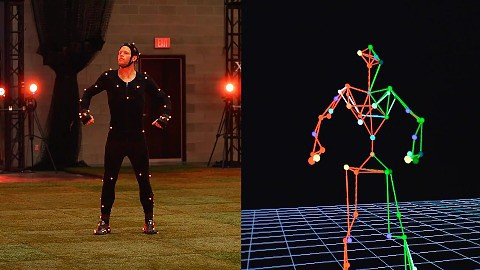
\includegraphics[width=\linewidth]{motion_capture_fifa.jpg}
    \caption{Motion Capture in der Filmproduktion}
    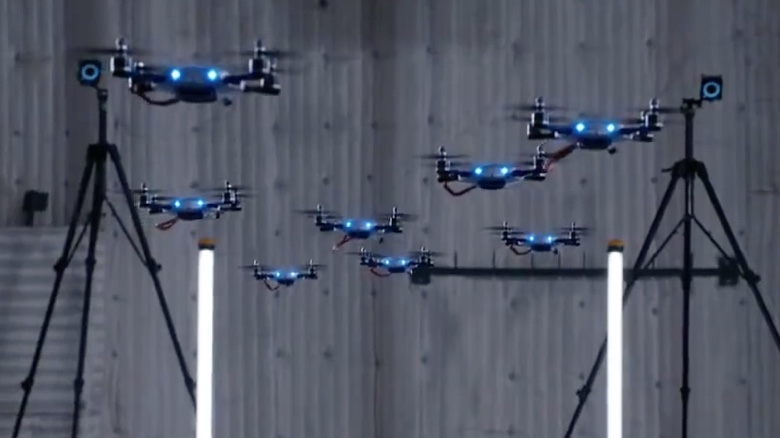
\includegraphics[width=\linewidth]{drones.jpg}
    \caption{Ein Schwarm von Drohnen kontroliert durch 3D-Tracking}
\end{wrapfigure}
In Filmen werden 3D-Tracking Systeme verwendet, um Bewegungen, Kämpfe und Szenen digital aufzuzeichnen und die gewonnenen Daten mit Hilfe computergenerierter Effekte zu den Szenen moderner Filme zu verwandeln, ohne die einzigartige Bewegungsart des Menschen zu verlieren (siehe Abbildung 1). 

Im Sport können Trajektorien eines Balles oder Bewegungen eines Spielers aufgezeichnet werden, um dem Training wichtige Informationen hinzuzufügen und auch in der Robotik ermöglicht das Tracking genau Steuerung und Korrektur von Drohnen oder Robotern. Nur durch die exakte Erfassung der Position können Fehler direkt oder im Voraus erkannt und korrigiert werden, die akkurate Positionierung und Bewegung des in Abbildung 2 zu sehenden Drohnen-Schwarm ist nur möglich, da eine zentrale Kontrolleinheit mithilfe der Daten aus einem 3D-Tracking-System die Bewegung der Drohnen hundertfach pro Sekunde anpasst. 
\subsection{Problematik}
\begin{wrapfigure}{r}{0.38\textwidth}
\centering
  {\setlength{\belowcaptionskip}{-10pt}
    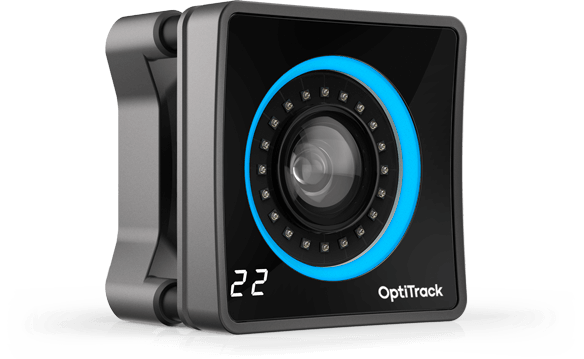
\includegraphics[angle=0,width=\linewidth]{4143.png}
    \caption{Optitrack UV-Tracking-Kamera}
  }
\end{wrapfigure}
Die Problematik, mit dem sich dieses Projekt befasst ist, dass es nur wenige Anbieter für solche Systeme gibt. Die Technik ist sehr teuer und nur gut finanzierte Projekte haben Zugriff auf diese revolutionären Systeme. Der bekannteste Anbieter Optitrack verlangt für die rechts gezeigt Kamera 4143\$, von denen für ein funktionierendes System mindestens 4 gebraucht werden. 

Das Ziel dieses Projektes ist es daher, ein Open-Source, günstiges und einfach zu integrierendes dreidimensionales Trackings-System zu entwickeln, damit Forscher, Entwickler und Interessierte auf der ganzen Welt, egal ob für Robotik, Filmproduktion oder der Messung von Bewegungen, 3D-Tracking als Basis für ihre Projekte verwenden können. \par
In dieser Projektarbeit wird die Theorie, der Entwicklungsprozess und die Ergebnisse meines 3D-Tracking Systems auf Basis herkömmlicher Webcams beschrieben und evaluiert.  
\newpage
\section{Vorgehen}
Bevor die tatsächliche Entwicklung der Software beginnen konnte, mussten zuerst die theoretische Funktionsweise und der grobe Aufbau des Systemes definiert werden.

\subsection{Theorie}
In einer Aufnahme einer herkömmlichen Kamera lässt sich die Position eines Objektes im zweidimensionalen Raum mithilfe von Object Tracking erfassen. Erweitert man diese Informationen mit den intrinsischen Werten der Kamera, also Brennweite, Verzerrung und Skalierung, in den dreidimensionalen Raum, fehlen einem die nötigen Informationen, um die Tiefe, also die Entfernung zur Kamera, zu berechnen.  

\begin{wrapfigure}{r}{0.38\textwidth}
\centering
  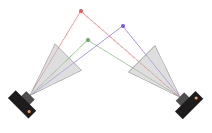
\includegraphics[angle=0,width=\linewidth]{triangulation.png}
  \caption{resultierenden Geraden zweier Perspektiven}
\end{wrapfigure}
Es bleibt also eine Gerade, auf der sich das Objekt befinden könnte. Wenn man nun eine zweite Kamera hinzufügt, erhält man eine weitere Gerade, auf der sich das Objekt befinden könnte. Liegen die Kameras an unterschiedlichen Orten, lässt sich die akkurate Position des zu trackenden Objektes durch den Schnittpunkt der beiden Geraden berechnen (siehe Abbildung 4). Wenn man jegliche Messfehler vernachlässigt, und die exakte Position der Kameras bekannt ist, würden zwei Kameras schon ausreichen, um die nötigen Daten zur Berechnung zu liefern.  

In der Realität gibt es aber einige Aspekte, die die Genauigkeit und Funktionalität des Systems negativ beeinflussen: 
\begin{itemize}
  \item Da ein Bild einer Kamera eine begrenzte Auflösung hat, kann eine Kante eines Objektes nur die Hälfte eines Pixels ausfüllen. Durch das „Auf- oder Abrunden“ dieser Bildinformationen entsteht ein Messfehler, der mit zunehmender Distanz größer wird. 
  \item Da die verwendeten Kameras  nur selten Informationen zu den intrinsischen Daten mitliefern, lassen sich diese nur mithilfe einer Kalibrierungssequenz ermessen. In der werden mehrere aufgenommen verzerrte Bilder so angepasst, dass sie den tatsächlichen Eigenschaften eines bekannten Objektes nahekommen, in der Praxis ist dies meist ein Schachbrett. In der resultierenden Projektion der Aufnahme im dreidimensionalen Raum können durch Messfehler Verzerrungen oder Verschiebungen entstehen. 
  \item Der mit Abstand stärkste Einfluss auf mögliche Fehler ist die durch eine Kalibrierungssequenz geschätzte Position der Kameras. Sowohl Rotation und Transposition zur Uhrkamera müssen perfekt sein, damit tatsächlich ein Schnittpunkt entsteht. 
\end{itemize}

Es wird also ersichtlich, dass ein perfekter Systemaufbau aufgrund der vielen Variablen nicht realistisch ist, und die Position des getrackten Objektes angenähert werden muss. Um diese möglichst nahe an die tatsächlichen Werte zu bringen, gibt es folgende Möglichkeiten: 
\begin{itemize}
  \item Eine größere und besser verteilte Anzahl an Kameras. Der kleinste Fehler für die Annäherung eines möglichen Schnittpunktes verschiedener Geraden entsteht dann, wenn diese orthogonal zueinander verlaufen. Es ist also vorteilhaft die Kameras möglichst effektiv im Raum zu positionieren. Auch die Anzahl verringert den Fehler, da einerseits mehr Daten entstehen und anderseits beim Ausfall oder starkem Messfehler nicht gleich das ganze System zusammenbricht. 
  \item Ein Algorithmus zum Erkennen von starken Messfehlern und guter Annäherung eines möglichen Schnittpunktes. 
\end{itemize}

\newpage
\subsection{Technische Voraussetzungen}
Bevor es an die tatsächliche Entwicklung gehen kann, müssen einige Spezifikationen, Voraussetzungen und zu verwendende Systeme definiert werden, damit das grobe Konzept auch tatsächlich umsetzbar ist. Dazu gehört die verwendete Hardware in Form von Kameras und Software in der Form von Programmiersprache, Bibliotheken und Programmen zur Entwicklung und Visualisierung. 

\subsubsection{Python}
Da das Projekt komplex ist, ist eine „high-level“ Programmiersprache zu präferieren, wodurch komplexere Aufgaben mit weniger Befehlen gelöst werden können. In diesem Bereich bietet sich Python besonders an, da diese einerseits großen Support in Form von zahlreichen Libraries und einer aktiven Community besitzt und ich andererseits bereits viel Erfahrung in diesem Bereich hatte. 

\subsubsection{ROS}
Das zu entwickelnde System sollte besonders variabel, erweiterbar und vielseitig nutzbar sein, es ist daher sinnvoll den Code modular aufzubauen, sodass bestimmte Teile ausgetauscht, verbessert oder erweitert werden können, ohne die Funktionalität des ganzen Systems zu hindern.  

Um eine solche Modularität schaffen zu können, werden bestimmte Vereinbarungen und Vorgaben gebraucht, wie zwischen Teilen kommuniziert werden soll, wie diese voneinander abhängig sind und wie die generelle Struktur des Systems aussieht.  

So wäre es beispielsweise sinnvoll, das Auslesen, Verarbeiten und Vergleichen der Kamerabilder voneinander zu separieren, sodass einerseits eine gewisse Unabhängigkeit entsteht und andererseits so von Multithreading Nutzen gemacht werden kann, der Aufteilung der Rechenlast auf mehrere CPU-Kerne.  

Auch wenn zahlreiche Lösungen für das Aufteilen eines Python-Programmes in verschiedene Threads (Unterprogramme) bereits nativ möglich ist, wäre die Integration in komplexere Systeme äußerst mühselig, da vor allem die Kommunikation in Form von geteilten Variablen eher primitiv und zeitlich aufwändig wäre. Es musste also ein System her, dass die Kommunikation und Separierung der Programme vereinfachen würde und idealerweise bereits vorgefertigte System für kleinere Aspekte des Projektes hätte, sodass bei der Entwicklung auf bereits getesteten Code zurückgegriffen werden konnte. 

\begin{wrapfigure}{r}{0.38\textwidth}
\centering
  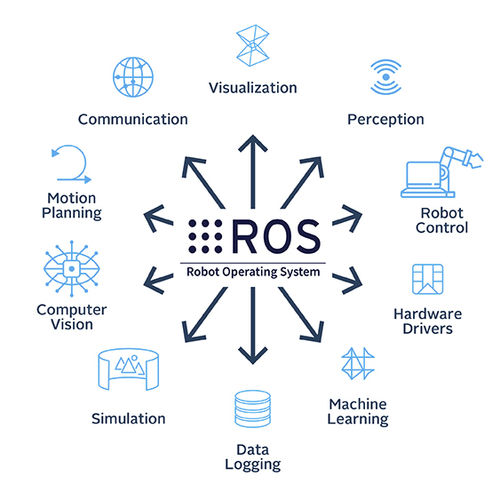
\includegraphics[angle=0,width=\linewidth]{ROS_diagram.jpg}
  \caption{Anwendungen von ROS}
\end{wrapfigure}
Alle diese Voraussetzungen erfüllte das Open-Source System „ROS“ (Robotic Operation System), ein seit 2007 entwickelte Framework für Roboter, welches in zahlreichen persönlichen und industriellen Systemen verwendet wird. ROS, oder im Falle dieses Projektes die zweite Version ROS2, ist weniger eine Library für eine bestimmte Programmiersprache, sondern wie im Namen schon enthalten, ein „Operating System“, also eine Vielzahl an Libraries, Tools und Algorithmen für die Entwicklung von Robotern, die tiefer im System integriert sind. Der Code selbst wird dann in Python geschrieben, und kann mithilfe einer Library (rclpy) mit ROS kommunizieren. 

ROS ermöglicht es nun, sogenannte „Nodes“ zu erstellen, diese sind unabhängige Module, die in ihrer eigenen Python oder C++ Datei erstellt werden können. So gibt es beispielsweise für jede Kamera eine Node, die sich nur um das Auslesen der Bilder kümmert, eine weitere zum Erkennen verschiedener Objekte und eine andere zum Vergleichen dieser Daten mit anderen Kameras.  

Allein können diese Module allerdings nichts erreichen, da sie von Informationen untereinander abhängig sind. Auch hier bietet ROS zwei zentrale Tools zur Kommunikation zwischen Nodes:  

\begin{itemize}
  \item Das Publisher-Subscriber Modell, in dem die Kommunikation stets nur in eine Richtung läuft. Wie in Abbildung 6 zu sehen, veröffentlicht der Publisher eine Nachricht mit bestimmten Parametern (Message) auf einem Topic, auf dem mehrere Subscriber "zuhören" können. 
  \begin{figure}[h]
    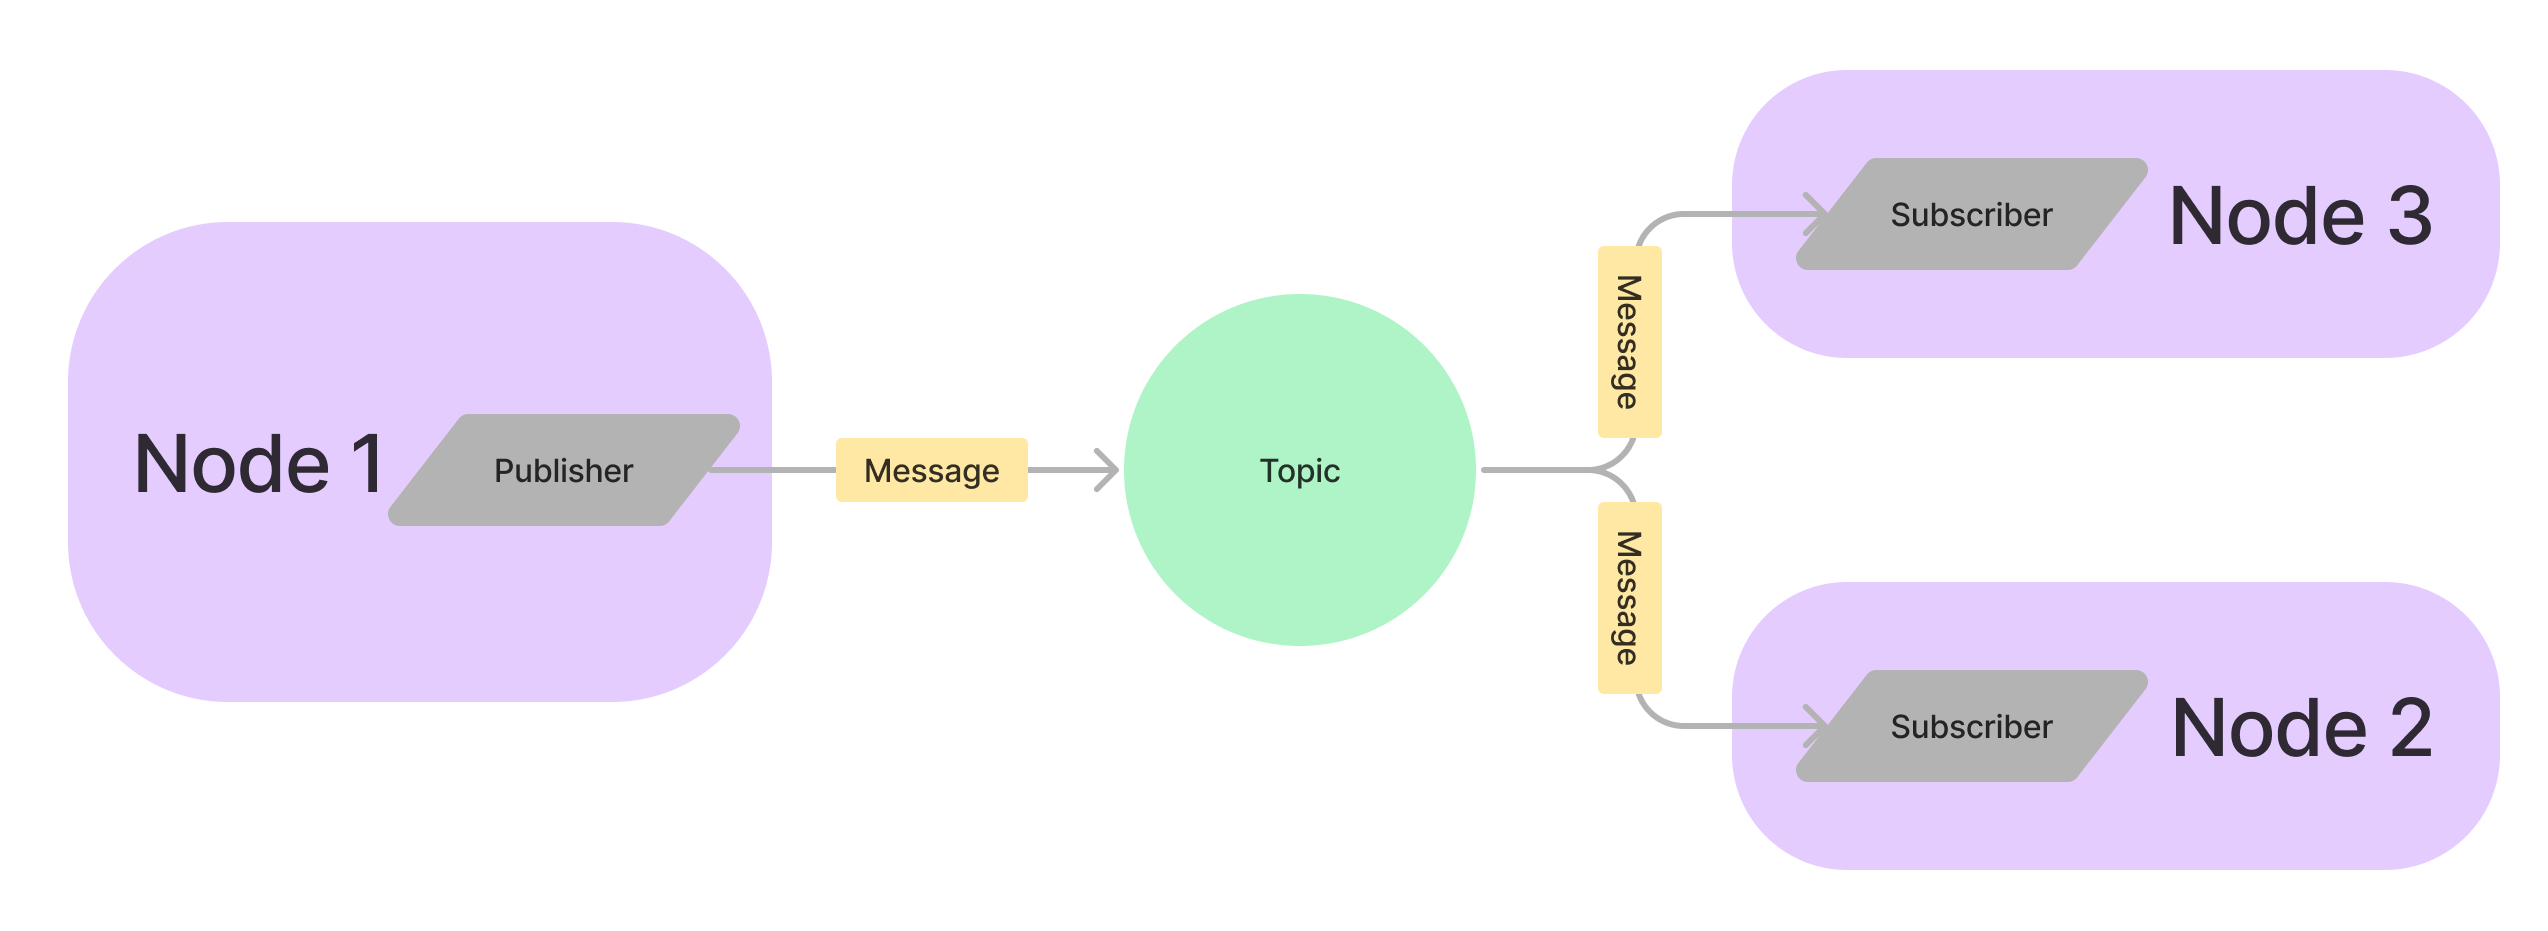
\includegraphics[angle=0,width=\linewidth]{Publisher.png}
    \caption{Publisher-Subscriber-Modell}
  \end{figure}
  \item Das Service-Modell, in dem die Kommunikation wie bei einem TCP-Handshake verläuft, also vom Client eine Anfrage zum Server gesendet wird und bei erfolgreicher interpretation eine Antwort zurück kommt. 
  \begin{figure}[h]
    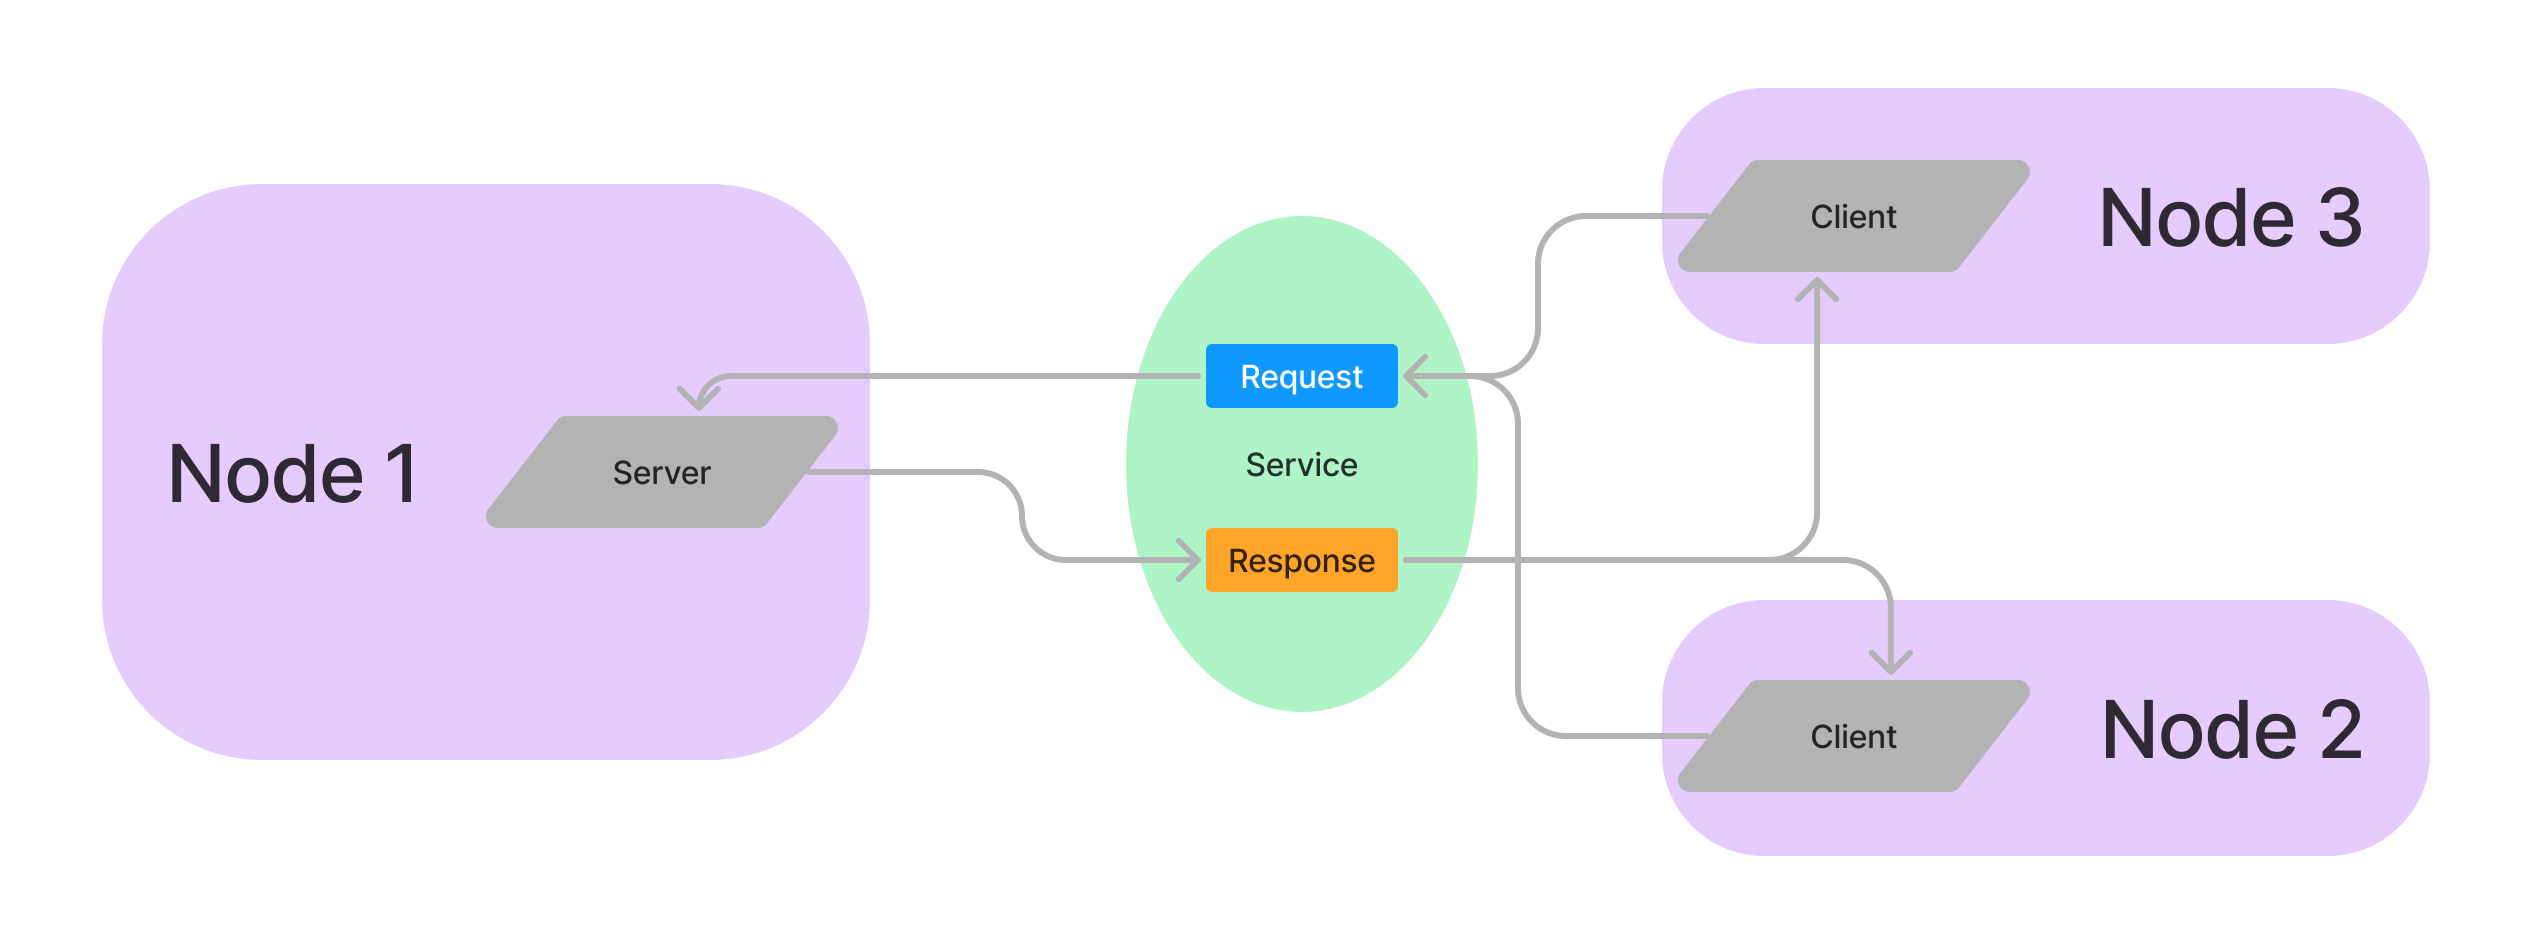
\includegraphics[angle=0,width=\linewidth]{Server.png}
    \caption{Server-Client-Modell}
  \end{figure}
\end{itemize}

Da alle Kommunikation meist einseitig sind und Geschwindigkeit eine wichtige Rolle spielt, wird im 3D-Tracking-System stets über das Publisher-Subscriber-Modell kommuniziert.

Ein weiterer Kernaspekt, weshalb ROS ein essenzieller Part dieser Entwicklung ist, hat mit der Etablierung der Technik zu tun. Da jede Art von Kommunikation durch sogenannte „Messages“ beschrieben wird, also welche Daten genau übertragen werden, gibt es viele Programme, die diese „verstehen“ können. Bilder, Vektoren, Kamera-Matrizen oder simple Punkte, werden daher immer auf dieselbe Weise versendet. So gibt es gute Möglichkeiten zur Visualisierung und Simulation der Daten, sowie zahlreiche andere Apps, die die Entwicklung durch ROS erleichtern. 
\subsubsection{Opencv}
Eine weitere Library, die in diesem Projekt eine große Rolle spielt, ist OpenCV, bzw. die Python Implementation. Dies ist eine freie Programmbibliothek mit Algorithmen für die Bildverarbeitung und Computer Vision. Durch sie wird sowohl das Auslesen der Kameradaten, als auch die Kalibrierung zur Berechnung der intrinsischen Parameter möglich.
\subsection{Vorgehensweise und Wandel}
Um die Flexibilität und Zuverlässigkeit des Systems sicherzustellen, wurde in der Entwicklung jedes Modul ausgiebig getestet, sowohl separat als auch im System integriert. Das Vorgehen in der Programmierung war also stets mit dem Testen des Systems verbunden, weshalb jedes Modul kontinuierlich im Laufe des Projektes verbessert wurde, sobald Fehler entdeckt wurden oder neu Funktionalität nötig war. 

\section{Systemaufbau}
Jede Ausführung des Tracking-Systems startet mit dem sogenannten "Manager", dies ist ein Programm, welches nach angeschlossenen Kameras sucht und alle nötigen Nodes zum Tracking konfiguriert und startet. Ein laufendes System kann in etwa so aussehen:
\begin{figure}[h]
  \centering
  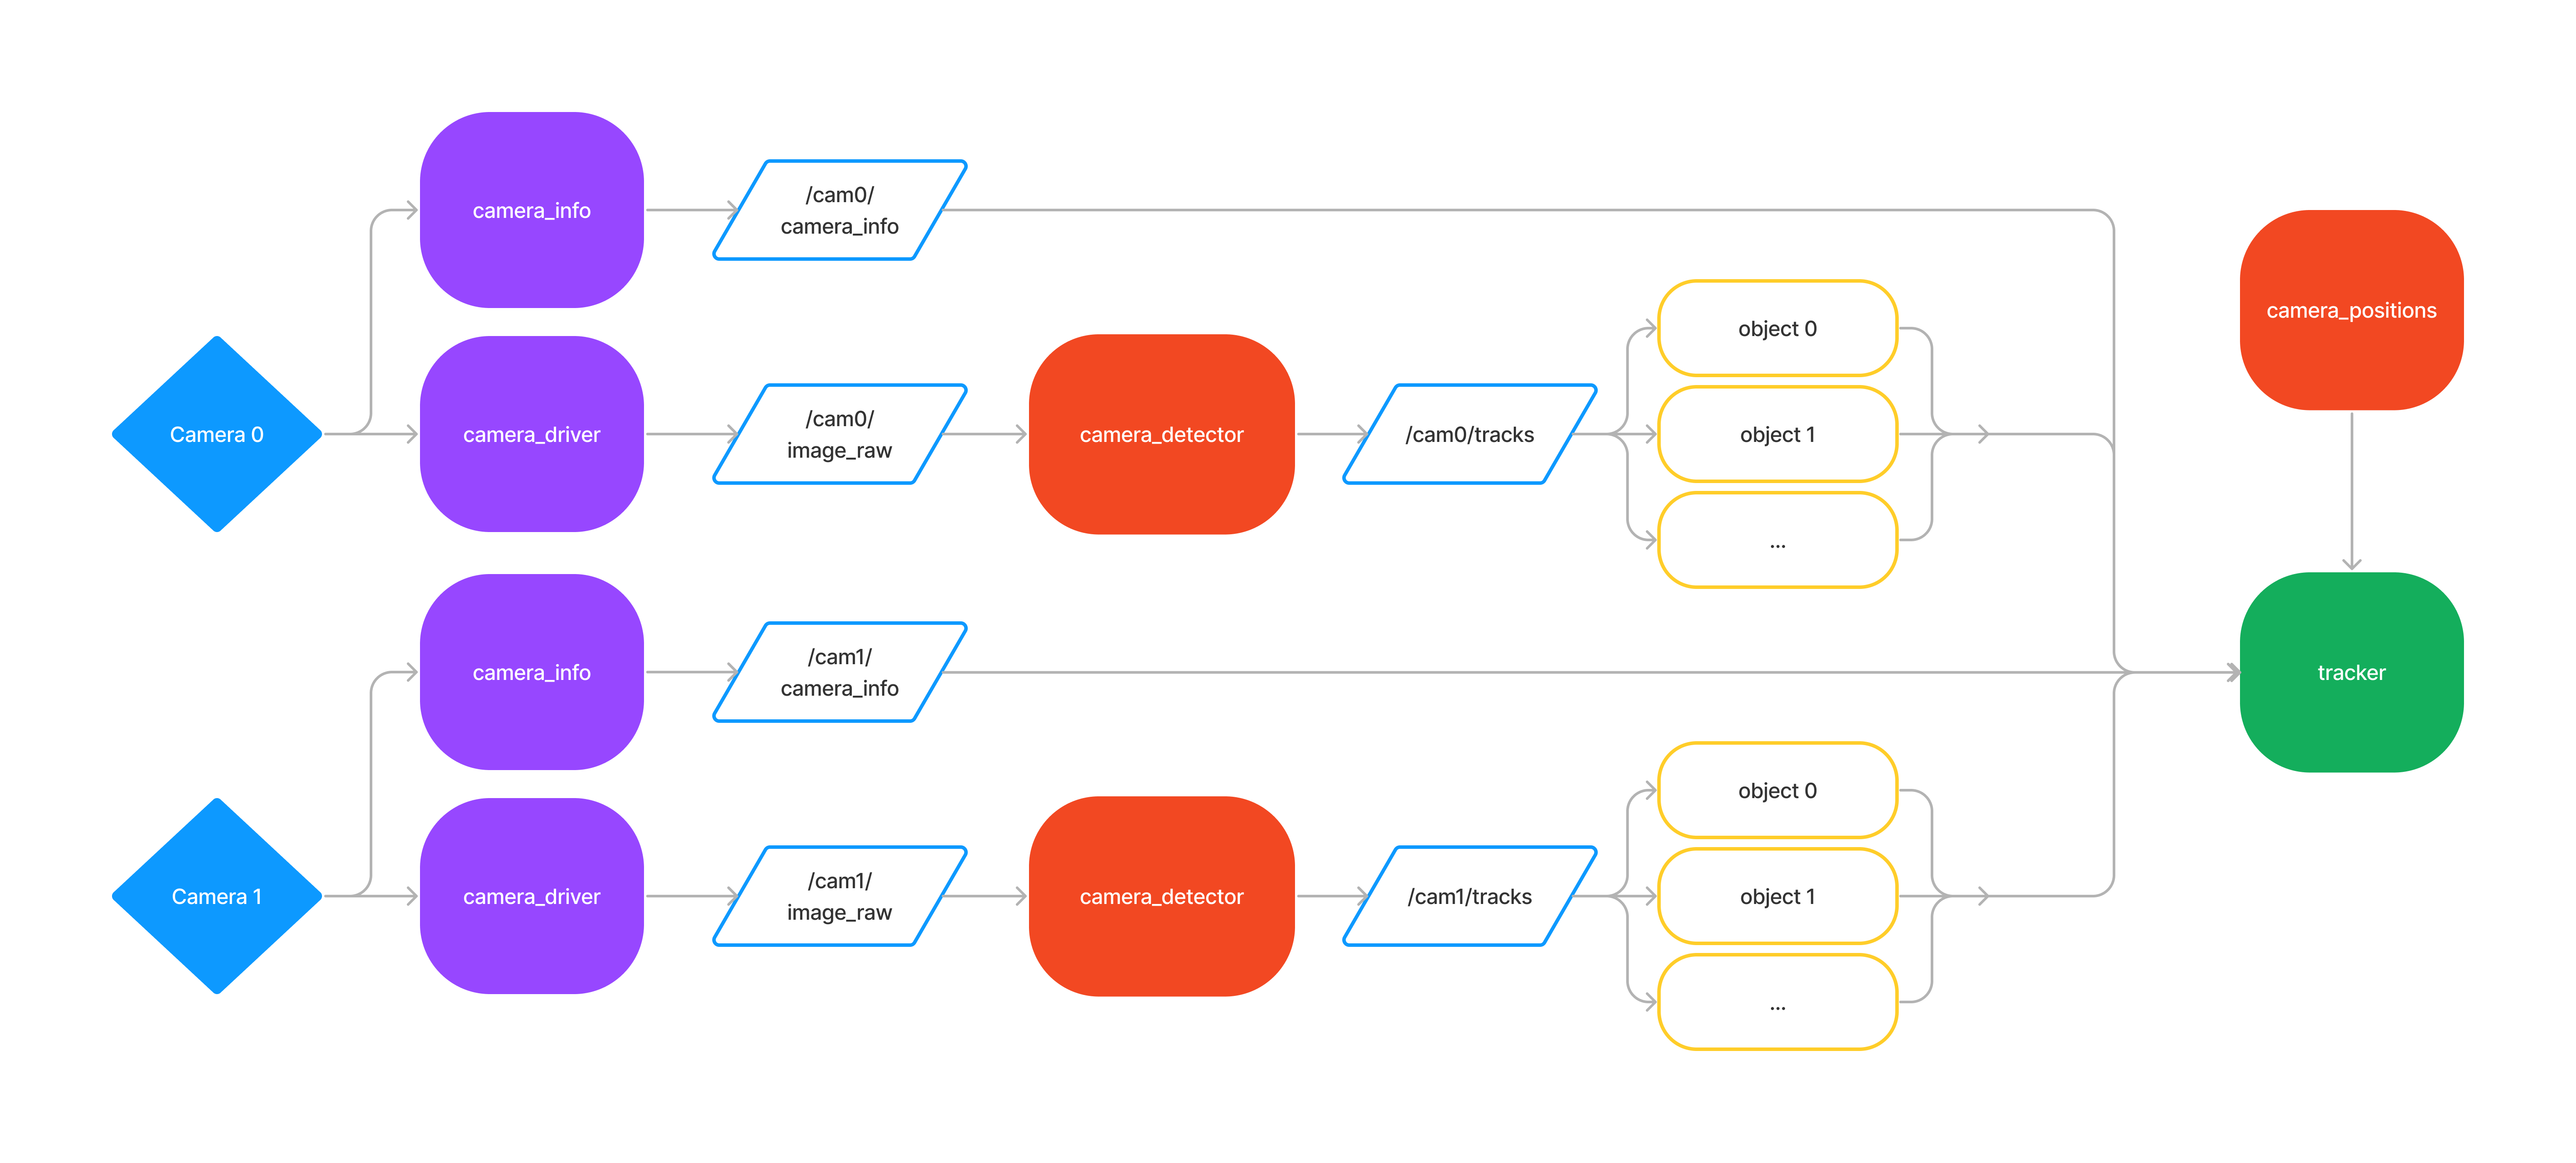
\includegraphics[angle=0,width=\linewidth]{anytrack-basic-tracking.png}
  \caption{Nodes, Topics und Messages eines laufenen Systemes mit 2 Kameras}
\end{figure}

Die Funktionalität und Aufgabe der einzelnen Module  wird im Folgenden erklärt:
\subsection{Driver}
Ursprünglich war das Auslesen und Verarbeiten der Bilder in einem Modul kombiniert, in dem eine kontinuierliche Schleife die Daten ausliest, verarbeitet und nach zu trackenden Objekten scannt. Im späteren Verlauf der Entwicklung zeigte sich jedoch, dass es nur durch die Separierung möglich ist, eine Simulationsumgebung möglichst direkt in das System zu integrieren. Dies ist nötig gewesen, da die Entwicklung des Kalibrierung-Prozesses zur Schätzung der Kamera Posen synthetische Daten gebraucht hat, um ein stabiles und stets identisches System zum Testen zu haben. 

Wenn die Bilder nicht von der Simulationssoftware gegeben werden, gibt der "camera\_driver" (siehe Abbildung 8) das Bild im ROS Netzwerk frei.

\subsection{2D-Tracking}
Bevor die Position eines Objektes im dreidimensionalen Raum berechnet werden kann, müssen erstmal die zweidimensionalen Koordinaten des Objektes im Bild der Kamera errechnet werden, wofür das "camera\_detector" Modul zuständig ist. Als Tracking-Objekt dienen kleine hellgrüne Kugeln, da sie von allen Seiten gleich aussehen und gut vom Hintergrund zu unterscheiden sind  

Üblicherweise wird für solche Zwecke Object-Tracking verwendet, bei dem die bestimmten visuellen Eigenschaften eines Objektes gespeichert und im nächsten Frame danach gesucht wird. Ein solches Objekt kann ein Auto, ein Mensch oder in diesem Fall eine Kugel sein.  

Auch wenn Object-Tracking mit Librarys wie OpenCV erstaunlich leicht zu integrieren ist, gibt es in diesem Fall eine simplere und schnellere Methode: Das Tracking von bestimmten Farb-Konturen, die nach dem Anwenden einer bestimmten „Maske“ übrigbleiben. 

Die Problematik bei dieser Technik liegt in der Unterscheidung des Objektes zum Hintergrund. In professionellen, aber sehr viel teuren Systemen, wird auf Infrarot-Kameras und besonders reflektierende kleine Kugeln gesetzt. Dieselbe Technik lässt sich aber auch auf herkömmlichen Webcams anwenden, wenn die Kugeln in einer besonders starken und im Hintergrund nicht vorhandenen Farbe sind. 

\vspace{10pt}
\begin{figure}[H]
  \begin{wrapfigure}{r}{0.4\textwidth}
    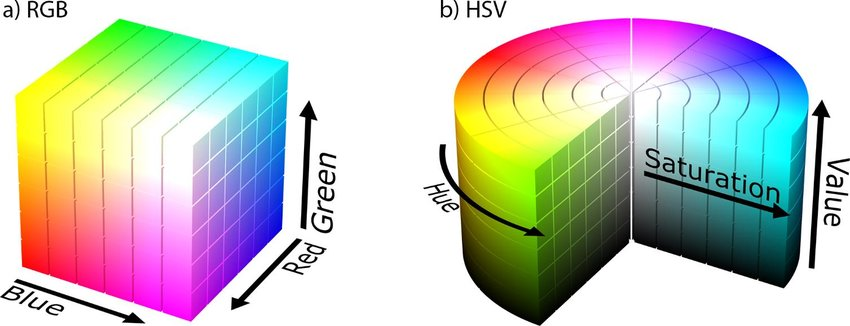
\includegraphics[angle=0,width=\linewidth]{rgb-hsv.png}
    \caption{RGB und HSV Farbformat}
    \label{Abb: HSV}
    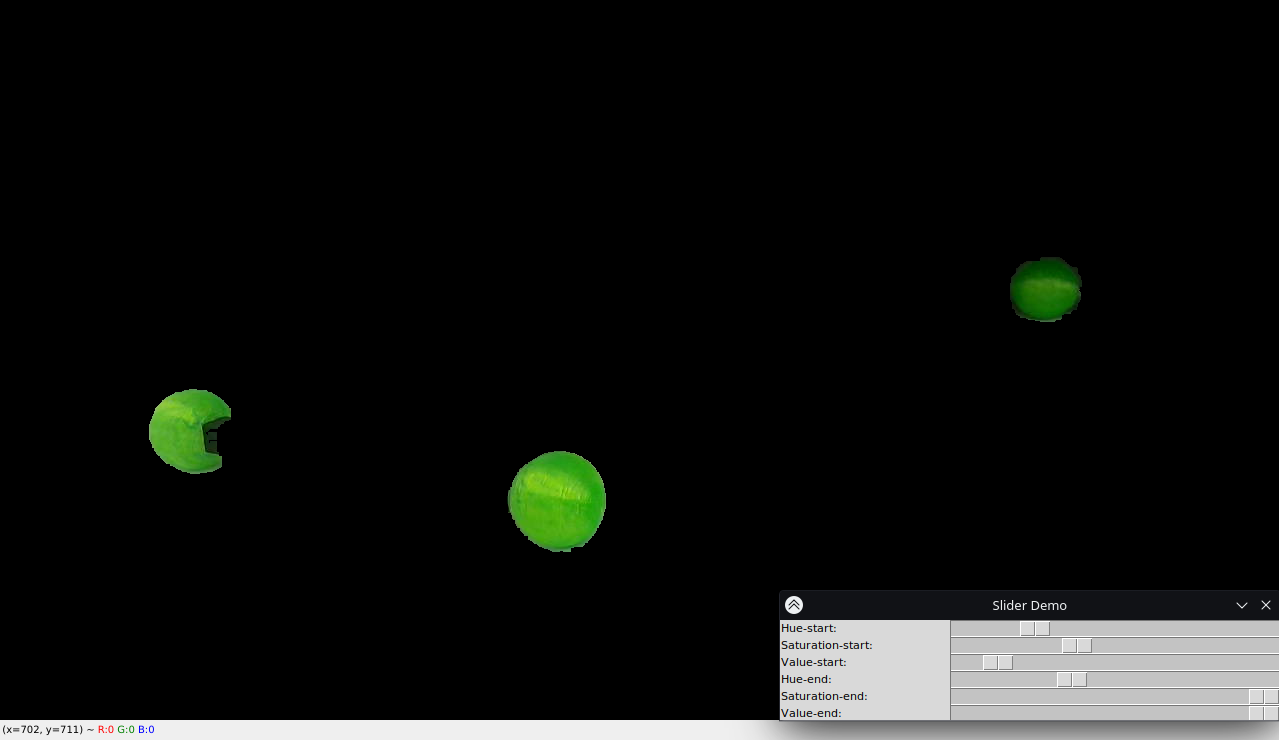
\includegraphics[angle=0,width=\linewidth]{2d-normal-filter.jpg}
    \caption{angewandter Farbfilter}
    \label{Abb: Farbfilter}
  \end{wrapfigure}
  Die Problematik bei dieser Technik liegt in der Unterscheidung des Objektes zum Hintergrund. In professionellen, aber sehr viel teuren Systemen, wird auf Infrarot-Kameras und besonders reflektierende kleine Kugeln gesetzt. Dieselbe Technik lässt sich aber auch auf herkömmlichen Webcams anwenden, wenn die Kugeln in einer besonders starken und im Hintergrund nicht vorhandenen Farbe sind. 

  Durch das Konvertieren des aufgenommenen Bildes vom RGB zum HSV-Format (siehe Abbildung \ref{Abb: HSV}), kann man die Daten so filtern, dass nur eine bestimmte Farbe übrigbleibt. Das HSV-Format ist dabei sehr nützlich, da ähnliche Farben (wie beispielsweise hell und dunkelgrün), nah einander liegen, und nur durch Filtern des Farbwertes (Hue), der Farbsättigung (Saturation) und dem Hellwert (Value), eine grobe Maske erstellt werden kann (siehe Abbildung \ref{Abb: Farbfilter}). 
\end{figure}

Beim Testen dieses Konzeptes stellte sich jedoch heraus, dass die Farbe allein nicht genug Kontrast ist, um die Kugel zuverlässig vom Hintergrund zu unterscheiden. Bei schlechter oder einseitiger Beleuchtung wurde die Farbe bestimmter Objekte signifikant dunkler, sodass die Filter, die am Tag funktioniert haben, nun gar nicht oder nur unzuverlässig funktionieren würden (siehe Kreise in Abbildung \ref{Abb: Lichtbedingungen}).  

\begin{figure}[htbp!]
  \centering
  \begin{subfigure}[t]{0.45\textwidth}
      \centering
      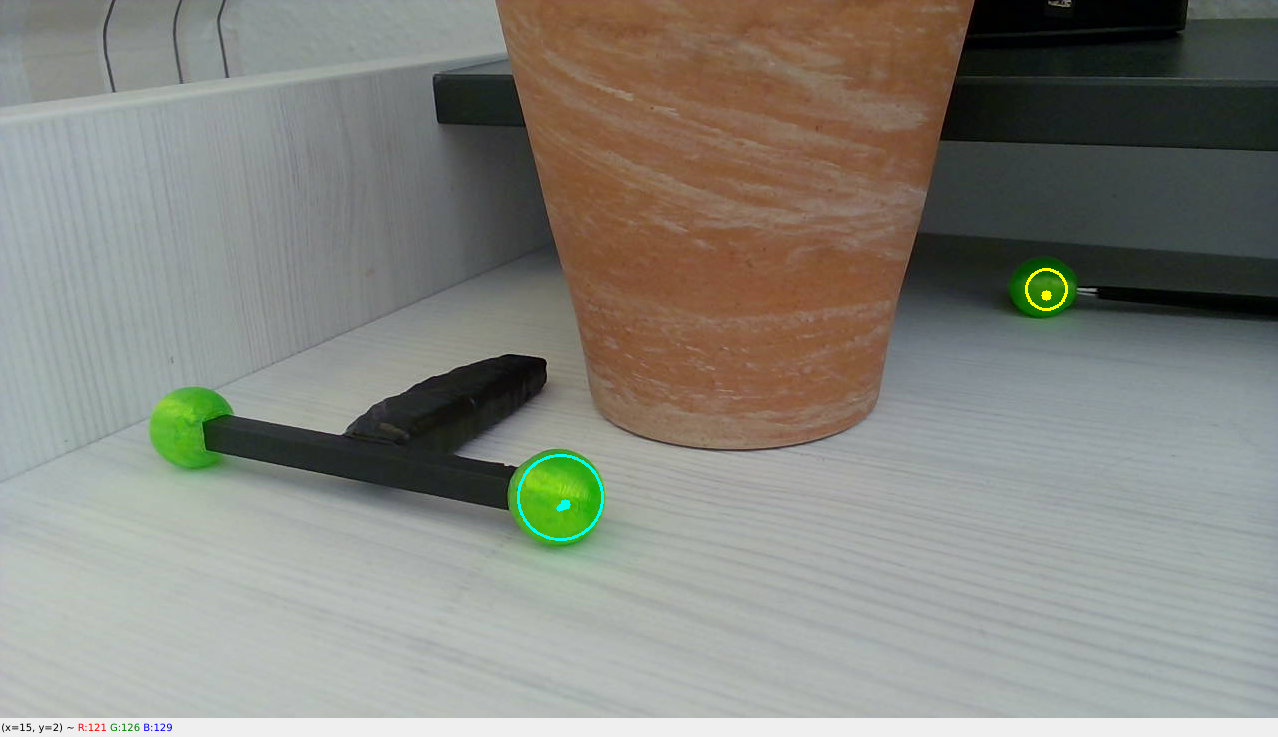
\includegraphics[width=\textwidth]{2d-normal.jpg}
      \caption{normale Lichtverhältnisses}
      \label{Abb: 2d-normal}
  \end{subfigure}
  \hfill
  \begin{subfigure}[t]{0.45\textwidth}
      \centering
      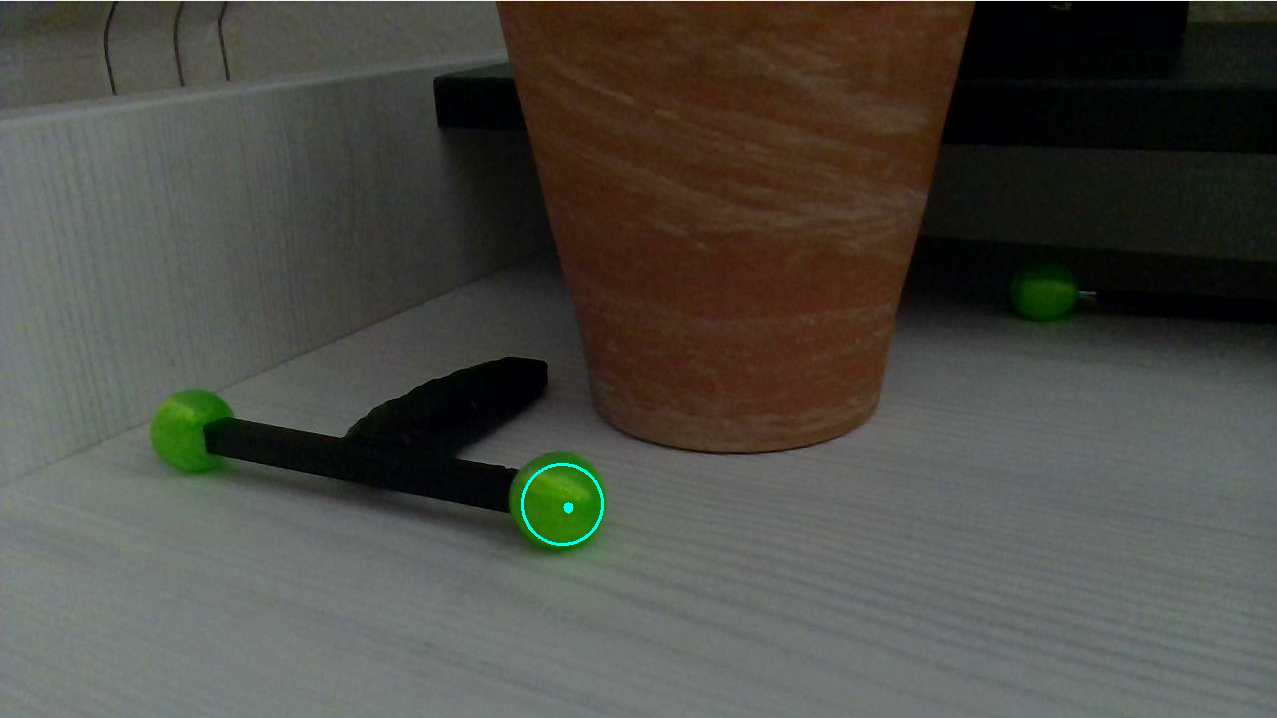
\includegraphics[width=\textwidth]{2d-normal-dark.jpg}
      \caption{dunkle Lichtverhältnisseschrieben}
      \label{Abb: 2d-normal-dunkel}
  \end{subfigure}
  \caption{Tracking Resultate in unterschiedlichen Lichtbedingungen}
  \label{Abb: Lichtbedingungen}
\end{figure}

\newpage
\begin{wrapfigure}{r}{0.35\textwidth}
  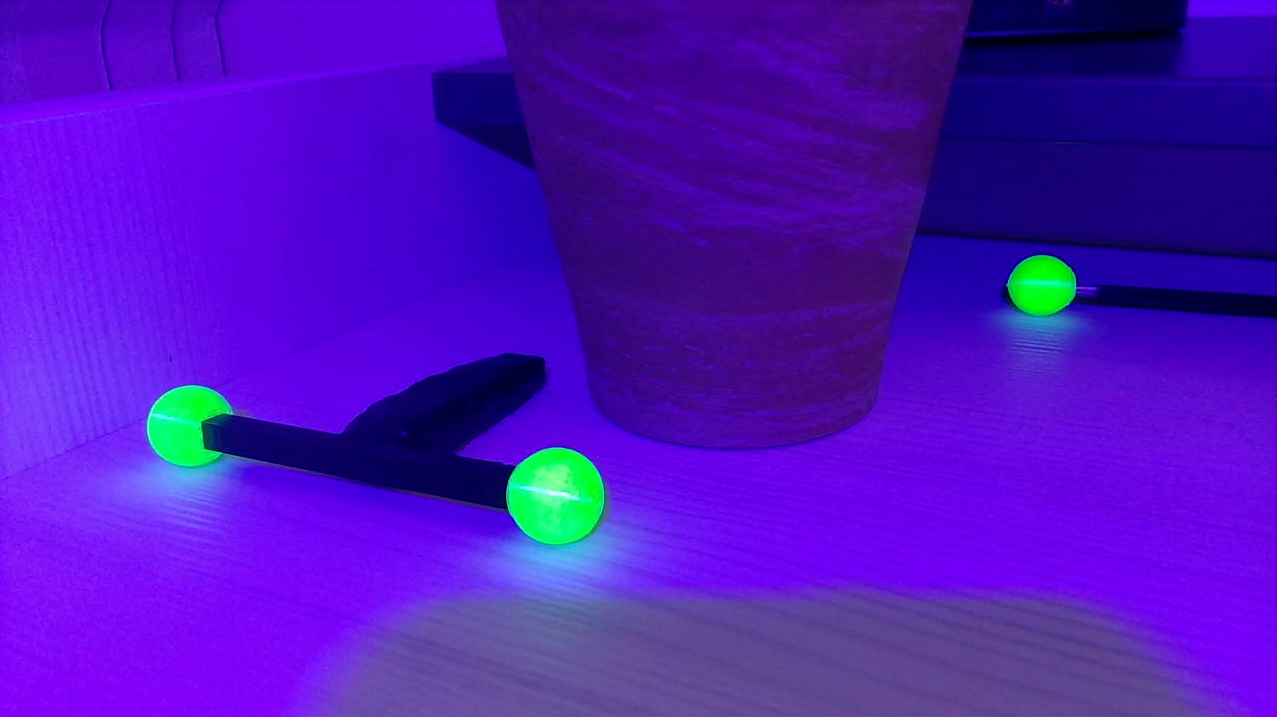
\includegraphics[angle=0,width=\linewidth]{2d-uv-normal.jpg}
  \caption{Farb-Maske nach Bildbearbeitungen}
  \label{Abb: UV}
\end{wrapfigure}
Die ursprüngliche Lösung für dieses Problem ist eine UV-Lampe gewesen, da das grüne Plastik der Kugel das umgangssprachlich genannte „Schwarzlicht“ stark reflektiert, und so stark von anderen Objekten im Raum unterschieden werden konnte. 

Auch wenn diese Lösung in gewissen Fällen funktioniert hat, musste die Stärke der Lampe und die Farbfilter für jede Umgebung neu eingestellt werden, um korrekt zu funktionieren. Ebenfalls war die Qualität des Trackings stark von dem Einfallswinkel des UV-Lichtes abhängig war. Würde dieses nämlich direkt in die Linse der Kamera reflektiert werden, was beim Auftreffen auf eine Kugel immer der Fall ist, würde dieser Bereich möglicherweise komplett weiß werden (siehe Abbildung \ref{Abb: UV}). Anders als Hellgrün ist Weiß eine Farbe, die immer im Hintergrund zu finden ist, und kann daher nicht in die Farbfilter mit integriert werden. 

Eine viel einfachere Lösung ergab sich durch das Experimentieren mit verschiedenen Bildbearbeitungen, die vor dem Tracking Algorithmus auf das Bild angewendet werden.  
Durch das Vermindern des Kontrastes und der Erhöhung der Sättigung sticht die Kugel nun viel stärker aus dem Bild hervor, und kann so deutlich einfacher mit einer Maske ausgeschnitten werden. Zudem verschwindet so der Kontrast zwischen den Seiten der Kugel, wodurch man einen stärker fokussierten Farbfilter verwenden kann, was Messfehler drastisch reduziert.  
Von der übrig gebliebenen Binär-Maske lässt sich relativ einfach das Zentrum einer Kontur und der Radius berechnen, indem eine Kreisform an die Konturen der einzelnen Masken angenähert wird, bis diese den Rand der Kontur erreicht. Durch diese Technik kann das Zentrum einer Kugel selbst dann
\begin{figure}[htbp!]
  \centering
  \begin{subfigure}[t]{0.45\textwidth}
      \centering
      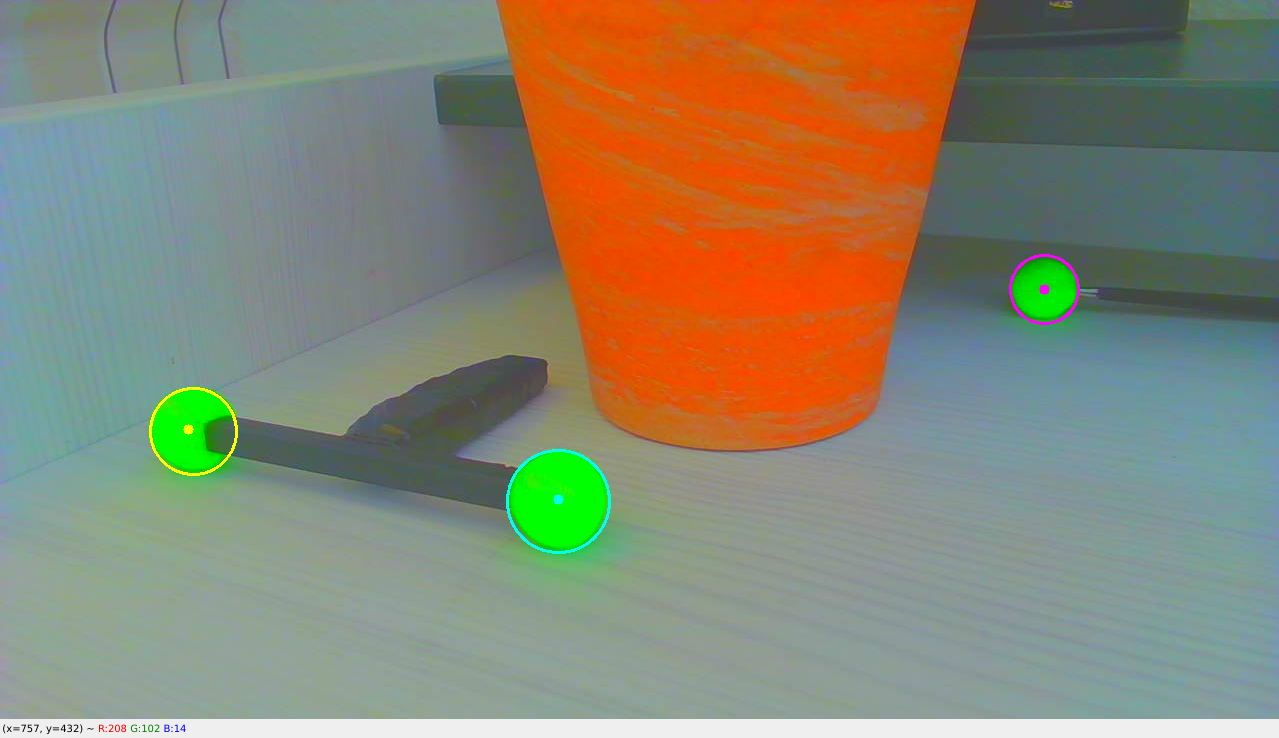
\includegraphics[width=\textwidth]{2d-color.jpg}
      \caption{normale Lichtverhältnisses}
      \label{Abb: 2d-color-normal}
  \end{subfigure}
  \hfill
  \begin{subfigure}[t]{0.45\textwidth}
      \centering
      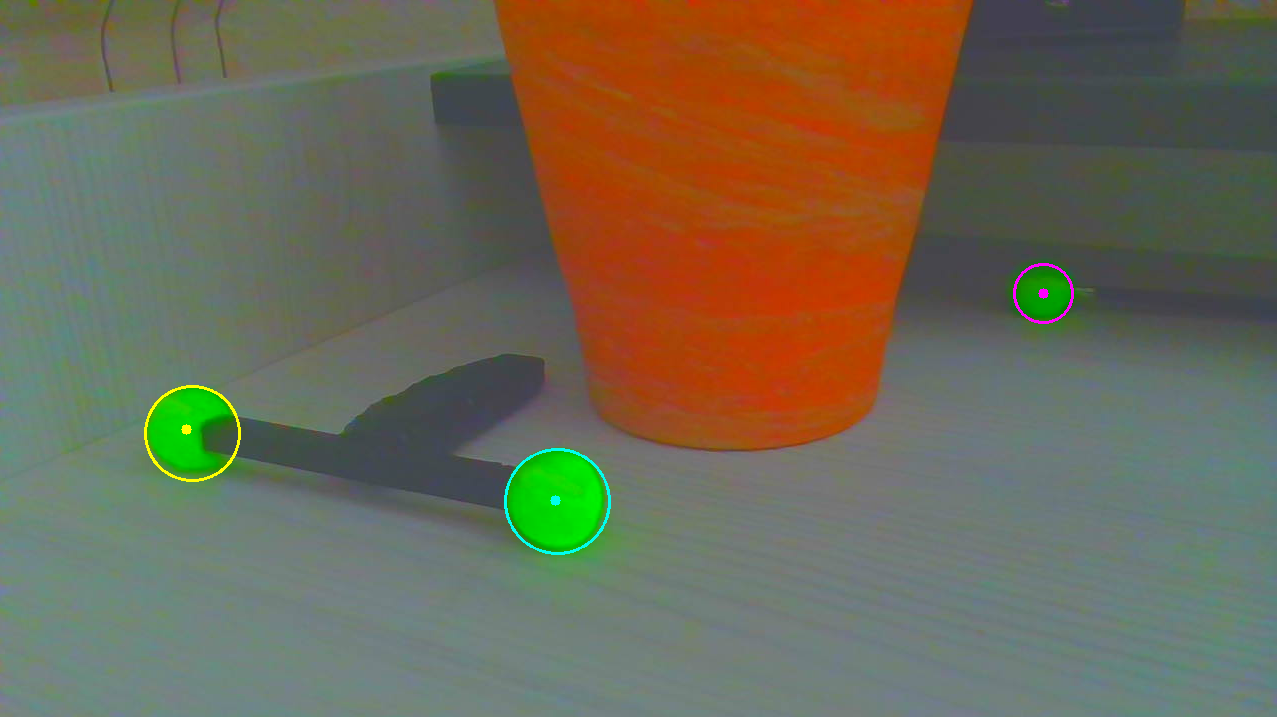
\includegraphics[width=\textwidth]{2d-color-dark.jpg}
      \caption{dunkle Lichtverhältnisseschrieben}
      \label{Abb: 2d-color-dunkel}
  \end{subfigure}
  \hfill
  \vspace{10pt}
  \begin{subfigure}[t]{0.6\textwidth}
      \centering
      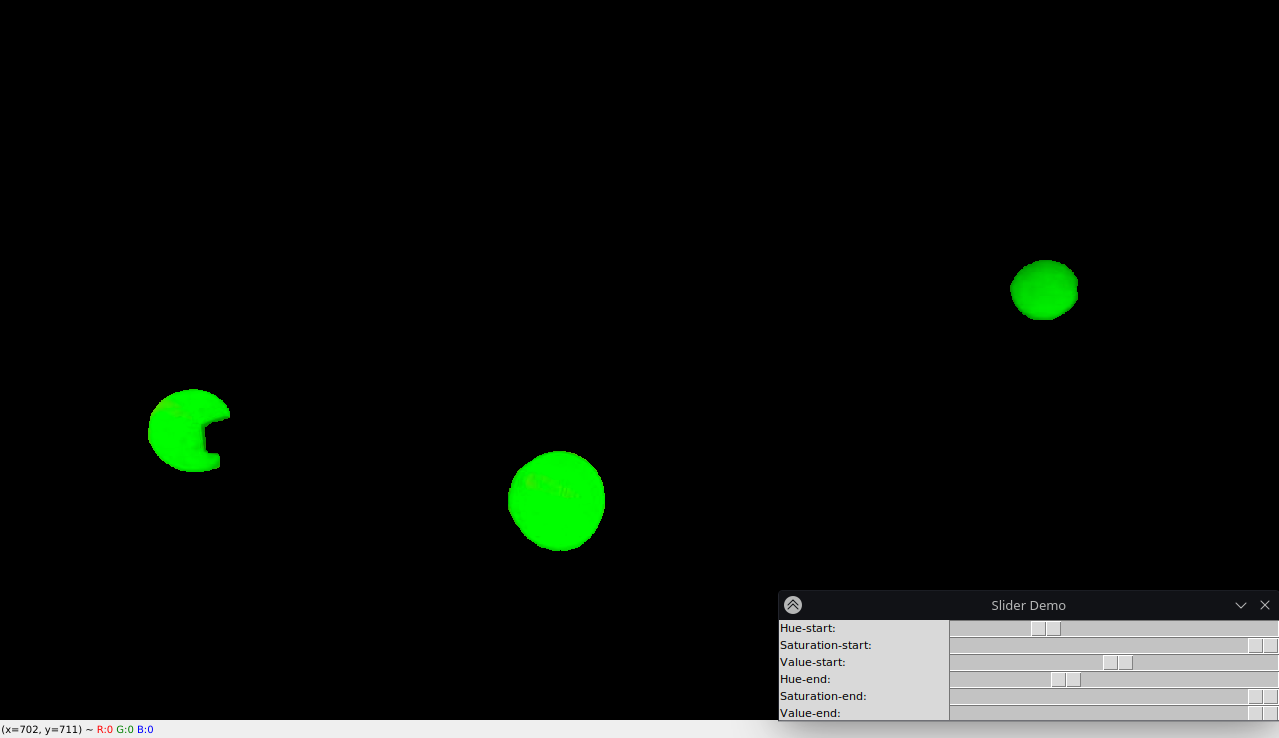
\includegraphics[width=\textwidth]{2d-color-filter.jpg}
      \caption{resultierende Maske}
      \label{Abb: 2d-color-maske}
  \end{subfigure}
  \caption{Tracking Resultate in unterschiedlichen Lichtbedingungen mit Nachbearbeitung}
  \label{Abb: Nachbearbeitungen}
\end{figure}

\subsubsection{Identifizierung der Objekt}
Auch wenn es für die meisten Anwendungen nicht nötig ist, können verschiedene Tracking Punkte durch zwei unterschiedliche Methoden im zeitlichen Verlauf und selbst in Bewegung voneinander unterschieden werden. Einerseits können mehrere Tracking-Farben hinzugefügt werden, zum Beispiel eine rote, blaue und grüne Kugel, andererseits vergibt der Tracking-Algorithmus jeder Kontur eine ID, und versucht im nächsten Frame diese anhand der Nähe zu den neuen Ergebnissen zum selben zuzuteilen. In der Praxis funktioniert die zweite Technik trotz ihrer Simplizität erstaunlich gut, sogar beim Überkreuzen zweier Laufbahnen.  

\subsection{Kamera-Kalibrierung}
Um die aus dem 2D-Tracking gewonnenen Daten in den dreidimensionalen Raum zu übertragen benötigt einige Information, die sich in intrinsische und externe Parameter gruppieren lassen. Ersteres sind dabei die Eigenschaften der Kamera selbst, also Brennweite, Verzerrung und Auflösung. Letzteres ist dabei vom 3D-Tracking-System konfiguriert. 
Der Rest der Parameter, die die Projektion eines 2D-Bildpunktes in den 3D-Raum beschreiben, müssen durch eine Kamera-Kalibrierung geschätzt und in folgende Berechnungen mit integriert werden. 

\subsection{3D-Vektoren}
\subsection{Positions-Kalibrierung}


\section{Ergebnisse}

\end{document}